\documentclass{article}[11pt]
%Required: You must have these
\usepackage{graphicx}
\usepackage{tabularx}
\usepackage{natbib}
\usepackage{caption}
\usepackage{subcaption}
\usepackage{array}
\usepackage{amsmath}
%\usepackage[backend=bibtex]{biblatex}
\setkeys{Gin}{width=0.8\textwidth}
%\setlength{\captionmargin}{30pt}
\setlength{\abovecaptionskip}{10pt}
\setlength{\belowcaptionskip}{10pt}
\topmargin -1.5cm 
\oddsidemargin -0.04cm 
\evensidemargin -0.04cm 
\textwidth 16.59cm
\textheight 23.94cm 
\parskip 7.2pt 
\renewcommand{\baselinestretch}{1.2} 	
\parindent 0pt

\bibliographystyle{..//..//refs/styles/besjournals.bst}
\usepackage{xr-hyper}
\usepackage{hyperref}
\externaldocument{suppliment}


\usepackage{lineo}
\linenumbers
\title{Biological and environmental drivers of flower-leaf sequence variation in the American Plums (\emph{Prunus}, sect. \emph{Prunocerasus}). }

\usepackage{Sweave}
\begin{document}
\input{outline-concordance}
\maketitle


\section*{Introduction}
%<<label=numbers, echo=FALSE, results=hide, message=FALSE>>=
%rm(list=ls()) 
%options(stringsAsFactors = FALSE)
%require(brms,quietly = TRUE)
%setwd("~/Documents/git/proterant/investment/Input")
%load("pcerasus.Rda")
%doyeff<-round(fixef(mod.ord.scale.phlyo)[6],digits=2)
%doyints<-round(fixef(mod.ord.scale.phlyo)[6,3:4],digits=3)
\noindent Woody perennials have a unique ability among plants to seasonally begin reproduction prior to vegetative growth. This flowering-first phenological sequence, known as hysteranthy, proteranthy or precocious flowering, is particularly common in temperate deciduous forests around the globe \citep{Rathcke_1985}. A number of studies suggest that this flower-leaf sequence (FLSs) is under selection, and that hysteranthy has functional significance, but the importance of variation in FLSs for maintaining fitness \citep{Gougherty2018,Buonaiuto2020,Guo2014} may vary across functional types and evolutionary clades within the temperate forest biome. With mounting evidence that anthropogenic climate change is driving shifts in flower-leaf sequences \citep{Ma2020:aa}, expanding our understanding of the adaptive benefit of hysteranthy is vital to forecasting the demography and performance of forest communities in an era of global climate change.

\noindent The most common, and well-tested explanation for the evolution of hysteranthy in temperate forests is that it is adaptive for wind-pollination, as leafless canopies increase wind speeds for pollen transport and reduce the likelihood of pollen interception by vegetation \citep{Whitehead1969,Niklas1985}. However, this explanation does not address the widespread prevalence of hysteranthy in biotically-pollinated taxa found in temperate regions. This number is not trivial; a recent analysis found that approximately 20\% of the hysteranthy species in the moist, Eastern Temperate Forests of North America are biotically pollinated \citep{Buonaiuto2020}. 

Several alternative hypotheses to the wind pollination hypothesis have been put forward to explain the advantage of hysteranthy in biotically-pollinated species, but they have not been widely evaluated in the literature. Below, we briefly review these hypotheses and their predictions, and then test these predictions using the American plums (\textit{Prunus} subspp. \textit{prunus} sect. \textit{prunocerasus}), a widespread clade with high variability in flower-leaf sequences as a representitive case-study. Our treatment here both clarifies the hypothesized function of flower-leaf sequence variation in biotically-pollinated taxa, and offers insights into how shifting flower-leaf sequences may impact species demography and distributions as climate continues to change.
%emwmar9 -- I like this opening!

%Despite the fact that  hysteranthous flowering in biotically-pollinated taxa violate (better word), the conventional explanation for this phenological syndrome, 

\subsection*{Hypotheses of Hysteranthous flowering in biotically pollinated taxa}

\underline{Water limitation hypothesis:} In the dry-deciduous tropics of South and Central America, hysteranthy is common \citep{Rathcke_1985,Franklin2016}, and is regarded as an important adaptation to alleviate water stress by partitioning the hydraulic demand of flowers and leaves across the season in this environment \citep{Gougherty2018,Franklin2016,Borchert1983,Reich1984}. By contrast,
temperate forests are rarely water-limited in the early season during which flowering and leafing occur \citep{Polgar2011}, but there is still considerable variation in water availability in space and time within temperate regions of the globe. Under this hypothesis, the function of hysteranthous flowering in these regions parallels that in the dry tropics---partitioning hydraulic demand across the season to allow hysteranthous species to tolerate increased aridity. If this is the case, we would expect to find hysteranthous taxa in locations that are, on average, drier than their non-hysteranthous relatives.

%\underline{Freeze tolerance hypothesis:} There is a demonstrated physiological relationship between drought and freeze tolerance, and it has been suggested that adaptations to drought allowed plants to expand their ranges higher latitudes of the Northern Hemisphere \citep{}. It is possible that hysteranthy contributed to this adaptation, though the mechanisms by which hysteranthous flowering may contribute to cold tolerance has not been investigated. One possibility is that for long lived organisms like woody plants, occasional frost damage to flowers has less of an impact on lifetime fitness, than damage to leaves (say better, I think I have old writing that might say this better). With this hypothesis, we would expect hysteranthous species to be found at colder sites than related non-hysteranthous ones. (Drop this if I don't have readily available data to test it.)
\underline{Insect-visibility hypothesis:} Hysteranthous flowers are visually conspicuous in the landscape. Thus, as in wind-pollinated taxa, hysteranthy in biotically pollinated taxa may be an adaptation for pollination efficiency as flowering-first species are easier for insects pollinators to locate \citep{Janzen1967}. This hypothesis predicts that hysteranthy should be associated with smaller floral displays, because flower are not obscured by leaves, they are easier to see, and there is weaker selection for increasing floral display size. %2) Hysteranthy may be associated with bigger flowers. Because these species are going all in on visual displays, big flowers might be additive to the benefits of hysteranthy. 
%emwmar9 -- I would love in my life to sneak in 'going all in' in a paper

\underline{Fruit maturaturion hypothesis:} There are several aspects of reproductive development that suggest hysteranthy is a by-product for early flowering, driven by development constraints. Hysteranthy may be common in large fruited species that require lots of time to mature their fruits, or in small, early fruiting species that have evolved dispersal syndromes (wind dispersal, non-dormant seeds) that require dispersal early in the season \citep{Primack1987}. In either case, we should expect fruit size to associate with hysteranthy.

Alternative to these functional hypotheses is the assertion that hysteranthous flowering is simply a by-product of selection for early flowering. Species that flower before their leaves inherently flower early in the season. Spring flower phenology is less constrained by prior phenological events than leaf phenology \citep{Savage2019}, which could allow selection to drive flowering into the early season, producing the hysteranthous phenological sequence. Here, there is no specific adaptive advantage to hysteranthy;  selection is not operating on the relative timing of flower and leaf emergence, but rather the absolute flowering time alone. If none of the predictions of the previously stated hypotheses are supported, this is the most likely null hypothesis.
 %emwmar9 -- below maybe works in discussion (mv from intro)? If not, just keep it short.DMB shortened it. 
%None of the hypotheses are mutually exclusive. One challenge is the same traits correlation could be driven by different mechanisms (i.e., small flower could be insect-visibility, developmental constraint, aridity tolerance or all of the above). Yet, a detailed investigation of the association between hysteranthy and the representative traits of each of these hypotheses would pinpoint those with the strongest theoretical underpinning and empirical evidence, as well as identify clear directions for future work to better understand the role that flower-leaf sequences play in woody plant fitness.

\noindent A significant challenge for robust testing of hysteranthy hypotheses is that most characterizations of flower-leaf phenological sequences are based on expert-opinion verbal descriptions (e.g. ``flowers before leaves" or ``flower before/with leaves"), which make comparisons across taxa, time and space difficult and sensitive to observer bias  \citep[see;][]{Buonaiuto2020}. This problem can be overcome by adopting standardized quantitative measures of plant phenology for observational studies and applying them to historic data records. Herbarium records are an excellent source of data that can be leveraged for quantitative phenological measurements \citep{Willis2017}, but have not be used widely to investigate variability of flower-leaf sequences variation among and within species.

The American plums offer potential for a high resolution investigation of drivers of hysteranthous flowering in taxa that are not easily explained by the dominant wind-pollination hypothesis. The 16 species that make up the section are distributed across the temperate zone of North America and, like the genus \textit{Prunus} at large, are all insect-pollinated, yet show pronounced inter-specific variation in flower-leaf sequences. Species in this section are well represented in herbaria records (Fig. \ref{fig:phylo2}a), making them a tractable group to measure and assess variation in flower-leaf sequences.

\noindent In this study we ask:\\

Do the observed associations between flower-leaf sequence variation and morphological and environmental traits match predicted associations of the hysteranthy hypotheses? 

\noindent First, we used herbaria records to to quantify both within- and across- species level variation in flower-leaf sequences of the American plums, (subspecies  \textit{Prunus}, sect. \textit{prunocerasus}).
Then we combined environmental attributes, biological traits and phylogenetic data in statistical models to interrogate the functional hypotheses for hysteranthous flowering described above. Finally, we compared our findings in this clade to patterns observed in larger genus \emph{Prunus} to better understand how phenology-trait associations vary over taxonomic scales.

%However, there are two major methodological challenges to testing the hydraulic demand hypothesis: First, characteristics like aridity tolerance, are the emergent product of a suite of biological traits \citep{Simova:2017vk}. Thus, when analyzing selective drivers of any particular trait at large taxonomic scales, unmeasured trait differences may obscure the estimated effects of the trait of interest, biasing results. This is a common problem in trait-based ecology, and one of the most promising solutions for understanding the functional significance of hysteranthy in woody plants is through character deconstruction \citep{Terribile2009}; comparing flower-leaf sequences variation for only a subset of taxa of shared phylogenetic and morphological character.   

%\noindent A second challenge for robust testing of hysteranthy hypotheses is that most characterizations of flower-leaf phenological sequences are based on expert-opinion verbal descriptions (e.g. ``flowers before leaves" or ``flower before/with leaves"), which make comparisons across taxa, time and space difficult and sensitive to observer bias  \citep[see;][]{Buonaiuto2020}. This problem can be overcome by adopting standardized quantitative measures of plant phenology for observational studies and applying them to historic data records. Herbarium records are an excellent source of data that can be leveraged for quantitative phenological measurements \citep{Willis2017}, but have not be used widely to investigate variability of flower-leaf sequences variation among and within species.

%Despite the pervasiveness of this phenological syndrome, direct tests of the function of hysteranthy in biotically pollinated taxa are rare for temperate forest species.
%but

%therefore


%. and in these ecosystems, flowering is associated with a recovery in plant water status due to leaf drop \citep{Borchert1983,Reich1984}. By temporally separating leaf and flower activity, woody plants can partition their hydraulic demand across the season, alleviating water stress \citep{Gougherty2018,Franklin2016}. 


%However, this hypothesis fails to address the prevalence of hysteranthous taxa that are biotically-pollinated. Approximately 30\% of woody plant species of Eastern temperate forests of North America flower before leafing out, and of these, approximately 20\% are biotically pollinated  \citep{Buonaiuto2020}. Despite the pervasiveness of this phenological syndrome, direct tests of the function of hysteranthy in biotically pollinated taxa are rare for temperate forest species.

%Yet looking to other biomes in which hysteranthous flowering is also common offers important insights regarding the function of hysteranthy in temperate, biotically-pollinated taxa. In the dry-deciduous tropics of South and Central America, flowering during the leafless period is also common \citep{Rathcke_1985,Franklin2016}. In these ecosystems, flowering is associated with a recovery in plant water status due to leaf drop \citep{Borchert1983,Reich1984}. By temporally separating leaf and flower activity, woody plants can partition their hydraulic demand across the season, alleviating water stress \citep{Gougherty2018,Franklin2016}. These physiological observations suggest that hysteranthous flowering may be an adaptation to arid environments.

%It is unclear whether this hydraulic demand hypothesis (also refered to as the water dynamic hypothesis \citep{Gougherty2018} or water limitation hypothesis \citep{Buonaiuto2020}) is relevant in the temperate zone where forests are rarely water-limited in the early season during which flowering and leafing occur \citep{Polgar2011}.%, and evidence of links between hysteranthy and aridity tolerance is mixed \citep{Gougherty2018,Buonaiuto2020} 
%Yet the hypothesis yields several predictions to evaluate whether hysteranthy serves to increase aridity tolerance in temperate flora:
%\begin{enumerate}
%\item Hysteranthous taxa should be found in dryer habitats compared to closely related, non-hysteranthous species.
%\item Hysteranthy may be linked to other reproductive traits associated with dry environments such as reduced flower and fruit size \citep{Herrera:2009aa,Liu:2013ua}.
%\item Additionally, flower-leaf sequences can be highly variable within individuals across time \citep{Buonaiuto2020}, and if hysteranthy contributes to aridity tolerance, climate variability may be positively correlated with variability in hysteranthy.
%\end{enumerate}
%\noindent With mounting evidence anthropogenic climate change is both driving shifts in flower-leaf sequences \citep{Ma2020:aa} and changing geographic patterns of water availability \citep{Overpeck11856}, understanding the functional significance of hysteranthy is vital to forecasting the demography and performance of forest communities in an era of global climate change. However, there are two major methodological challenges to testing the hydraulic demand hypothesis:

%\noindent First, characteristics like aridity tolerance, are the emergent product of a suite of biological traits \citep{Simova:2017vk}. Thus, when analyzing selective drivers of any particular trait at large taxonomic scales, unmeasured trait differences may obscure the estimated effects of the trait of interest, biasing results. This is a common problem in trait-based ecology, and one of the most promising solutions for understanding the functional significance of hysteranthy in woody plants is through character deconstruction \citep{Terribile2009}; comparing flower-leaf sequences variation for only a subset of taxa of shared phylogenetic and morphological character.   

%\noindent A second challenge for robust testing of hysteranthy hypotheses is that most characterizations of flower-leaf phenological sequences are based on expert-opinion verbal descriptions (e.g. ``flowers before leaves" or ``flower before/with leaves"), which make comparisons across taxa, time and space difficult and sensitive to observer bias  \citep[see;][]{Buonaiuto2020}. This problem can be overcome by adopting standardized quantitative measures of plant phenology for observational studies and applying them to historic data records. Herbarium records are an excellent source of data that can be leveraged for quantitative phenological measurements \citep{Willis2017}, but have not be used widely to investigate variability of flower-leaf sequences variation among and within species.

%\noindent In this study,we used herbaria records to to quantify flower-leaf sequence patterns in the American plums, (subspecies  \textit{prunus}, sect. \textit{prunocerasus}. We then evaluated the association between hysteranthy and several ecological and morphological traits to test the predictions of the hydraulic demand hypothesis of hysteranthy. Our findings both clarify the hypothesized function of flower-leaf sequence variation in biotically-pollinated taxa, and offer insights into how flower-leaf sequences may impact species distributions as climate continues to change.


%<<>>=
%mich.data<-read.csv("..//..//sub_projs/MTSV_USFS/michdata_final.csv")
%table(mich.data$pro2,mich.data$Pollination)

%table(mich.data$pro)
%42/147
%table(mich.data$pro2)
%82/147



\section*{Methods} %emwmar9 -- methods needs some typos help
%\subsection{Study system}
%\noindent The genus \texit{Prunus} comprises approximately 200 species distributed across the globe \citep{Chin:2014wu}, Within the genus, The American plums (\textit{Prunus} subspp. \textit{prunus} sect. \textit{prunocerasus}) offer potential for a higher resolution investigation of drivers of hysteranthous flowering. The 16 species that make up the section are distributed across North America and, like the genus \textit{Prunus} at large, show pronounced inter-specific variation in flower-leaf sequences. While within the larger genus species can be separated into three distinct morphological clades by inflorescence architecture (solitary, corymbose or racemose) all members of the section share solitary inflorescences \citep{Shaw:2004aa} allowing for refined character deconstruction. Species in this section are well represented in herbaria records (Fig. \ref{fig:mappy}), making them a tractable group to measure and assess variation in flower-leaf sequences as well as other ecological and morphological characteristics related to the hydraulic demand hypothesis. 

\subsection{Quantifying flower-leaf sequence variation}  %emwmar9 -- make sure methods and results are past tense
We obtained digital herbarium specimens for all members of the section \textit{Prunocerasus} from the Consortium of Midwest Herbaria (CMH) Database \citep{add citation}. To quantify flower-leaf sequence variation within and across species we randomly sampled 200 specimens for each species and scored the phenological development of flowers and leaves using a modified BBCH scale for woody plants \citep{Finn2007}. In total, we evaluated the phenology of 2521 specimens, but only specimens with visible flowers were included in this analysis (n=1009). We reconstructed the phylogenetic relationships among species in this group based on the tree topology in \citet{Shaw:2004aa}. We inferred branch lengths following the method of \citet{Granfen1989}in which node heights are estimated in proportion to number of subtending taxa using the R package ``ape" \citep{Paradis2019}.%  Following the methods of \citet{Granfen1989}, we computed branch lengths for this phylogeny by assigning each node a height and computed the distance between upper and lower nodes.
%\textit{Need to write this part more professionally}. To compute a phylogentic signal for flower-leaf sequence variation, we calculated the mean of the log(vegetative BBCH observed during flowering) for each species and calculated Bloomberg's K using the function phylosig \citep{}. 

To quantify FLS variation, we fit an ordinal, hierarchical, Bayesian, phylogenetic mixed model \citep{Garamszegi2014} to assess the likelihood an individual would be at any given vegetative BBCH phase while flowering. Our model predicted leaf stage (Y, ordinal with up to j categories) as a function of species and additional phylogenetic effects. Because hysteranthy co-varies with flowering time (i.e., flowering first species will generally flower earlier than other species, on average) we included day of observation as an additional predictor. The model is written below:\\

$logit(P(Y \leq j)) &= \alpha_{[j]phylo[i]}+ \alpha_{[j]sp[i]}+ \beta_{day of year[sp[i]]}*X_1+ \epsilon_{i}$\\
  
   \epsilon_i & \sim N(0,\sigma^2_y) \\ 
   
where Y is the ordinal outcome (leaf stage) and j is the number of categories (1,2,...6). $P(Y \leq j))$ is the probability of $Y$ less than or equal to a category $j&=1...j&-1$. $\alpha_{[j]}$ describes an intercept for each category [1,2,...6], while slope $beta_{\text{day of year}[sp[i]]}$ is constant across categories. 
  
  \noindent The influence of the phylogeny $\alpha_{phylo}$ was modeled as follows:\\
  \alpha_{sp} & \sim N(\mu_{\alpha}, COR[\sigma^2_{phylo}]) \\
  
  \noindent The $\alpha$ for species effects independent of the phylogeny was modeled as follows:\\
  \alpha_{sp} & \sim N(\mu_{\alpha}, \sigma^2_{species}) \\

 %We fit the model in the R package ``brms" \citep{Burkner2018} using weakly informative priors, and ran the model on four chains with a warm-up of 3,000 iterations and 4,000 sampling iterations for a total of 4,000 sampling iterations. Model fit was assessed with Rhats <1.01 and high effective sample sizes and no divergent transitions.
 
%Because the day of observation strongly influenced the BBCH stage likelihood, quantifying flower-leaf sequences among species was intractable without accounting for this temporal trend. To address this issues,
We used our model to predict the likelihood each species would be observed at a given vegetative BBCH stage during flowering at the 0\%, 25\% 50\% and 75\% quantiles of their flowering period. We then developed a flower-leaf sequence index, by assigning a numerical score to each species per seasonal quantile, and summing over the full flowering season. In each seasonal quantile, species received a ``1" if more than 50\% of their probability distribution occurred at the two earliest stages of vegetative phenology---BBCH 0 (``bud development") and BBCH 09 (``bud break")---and a ``0" if not. We summed these values across the season, generating an index from 0 (never hysteranthous) to 4 (hysteranthous through late season (Q75)), where 1&= hysteranthous at start of season, 2&= hysteranthous through early season  (Q25) and 3 &= hysteranthous through mid season (Q50). We also used two alternative indexing schemes ($>$25\% of the probability distribution occurred at BBCH 0 and $>$40\% of the probability distribution occurred at BBCH 0 and BBCH 09) to make sure our result were robust across multiple cutoffs.

\subsection{Evaluating hysteranthy hypotheses}

To test the predictions of the hypotheses we obtained data on petal length and fruit diameter directly from herbarium specimens. To assess aridity tolerance, we computed the average Palmer Modified Drought Index score from 1900-2017 for every \textit{Prunocerasus} specimen in the database (n=2305) from the North America Drought Atlas \citep{Cook2004}. For any specimens that lacked accurate geo-location information, we extracted PDSI values at the county centroid of the herbaria specimen. 

\noindent For our morphological measurements, we sampled an additional 321 specimens and measured the petal length of up to 10 randomly selected petals per specimen (n=2757) using ImageJ image processing software. We also used ImageJ to measure the diameter of fruits on an additional 316 specimens, measuring up to 5 fruit per specimen (n=224).

We then used Bayesian phylogenetic mixed models to test the relationship between flower-leaf sequence index scores and each of the variables. In these models, we modeled species and phylogeny as above. 

The model structure is written below: 

  y_i &= \alpha_{ind/sp[i]} +\alpha_{phylo[i]} + \beta_{hyst.index}*X_{hyst.index} + \epsilon_i\\
  
  \epsilon_i & \sim N(0,\sigma^2_y) \\ %Check this
  
  where Y is observed trait values (PDSI, petal length or fruit diameter), and the slope $\beta_{\text{hyst.index}$ describes the relationship between extended hysteranthy (higher hysteranthy index value) and the trait of interest. \alpha_{ind/sp[i]}  and \alpha_{phylo[i]} describe the species and phylogenetic effects respectively.  We also ran each model using our two alternative FLS indexing approaches to make sure our particular indexing approach was not influencing our results. Though these alternative classification schemes did change the hysteranthy index score for some species (Fig. \ref{fig:plums}), they did not substantially impact the inference from our models (see Tab. \ref{tab:modput} for comparisons).
  
 % \noindent The effect of the phylogeny was model as above.% and here, the individual effects within species were modeled:\\
  %alpha_{ind/sp} & \sim N(\mu_{\alpha}, \sigma^2_{ind/sp}) \\
  
%As above, we fit these models in the R package ``brms" \citep{Burkner2018} using weakly informative priors. We ran the models on four chains with a warm-up of 3,500 iterations and 4,500 sampling iterations for a total of 4,000 sampling iterations. Model fit was assessed with Rhats $<$1.01 and high effective sample sizes and no divergent transitions.

\subsection*{Hysteranthy in the larger genus \textit{Prunus}}

To better understand how the patterns we identified in our in-depth study of the \textit{Pruncerasus} clade scaled across coarser taxonomic resolution we also evaluated the relationship between hysteranthous flowering and hypothesis-related traits in all of the \text{Prunus} species that are native to, or established in North America. For this analysis, we obtained categorical descriptions of flower-leaf sequences and mean estimates of fruit diameter and number of flowers/inflorescence as a proxy for floral investment from the Flora of North America \citep{add citation} for 32 species in the genus.  We extracted PDSI values for all herbaria observation of those species in the Consortium of Midwest Herbaria database (n=23,272) as described above.

 
To account for the influence of evolutionary relationships among species, we reconstructed the phylogenetic relationships in the genus based on the tree topology in \citet{Chin:2014wu}. As as above, we computed branch lengths with the R package ``ape" \citep{Paradis2019}. 

We standardized the units of all predictors to make their effect size estimates for the following model structure directly comparable to each other: 

$logit(P(Y \leq j)) &= \beta_{[j]phylo[i]}+ \beta_{pdsi[sp[i]]}*X_1+\beta_{fruit diamter}*X_2+
+\beta_{floral investment}*X_3+\epsilon_{i}$\\
  
   \epsilon_i & \sim N(0,\sigma^2_y) \\ 
   
   where Y is the ordinal outcome of flower-leaf sequence category (``flowers before leaves",``flowers before/with leaves", ``flowers with leaves" and ``flowers after leaves") and j is the number of categories (1,2,...4). $P(Y \leq j))$ is the probability of $Y$ less than of equal to a category $j&=1,...j&-1$. We modeled the influence of the phylogeny ($\alpha_{phylo}$) as above.
%  In this varying slope and intercept model, $\beta_{[j]}$ describes an intercept for each category [1,2,...4].

\subsection{Model runs} 
 
We fit all models in the R package ``brms" \citep{Burkner2018} using weakly informative priors, and ran the model on four chains.
For the ``Quantifying flower-leaf sequence variation" and ``Evaluating hysteranthy hypotheses" we ran the models with a warm-up of 3000, and 3500 iterations, and 4000, and 4500 sampling iterations respectively, for a total of 4000 sampling iterations across all chains. For the ``Hysteranthy in the larger genus \textit{Prunus}" model, we used a warm up of 6,000 iterations and 8,000 sampling iterations for a total of 8,000 sampling iterations to maximize the effective sampling size. Model fits was assessed with Rhats <1.01, high effective sample sizes and no divergent transitions.
%\noindent Because our data dependent and independent were collect we employed a sequential modeling approach to first estimate the mean and standard error of the posterior distribution of trait values for each species then model the relationship between these estimate and the likelihood of hysteranthy using Bayesian measurement error models. This approach propagates the error in the initial estimates of trait values into the our final model, yielding a more accurate evaluation than using mean trait values alone \citep{}. For each parameter of interest, we ran Bayesian phylogenetic mixed-effects models with our measured traits as the response variable and species as the random effect. For traits like flower petal length and fruit diameters than included multiple measurements per specimen, we included specimen ID as an additional random effect. The model structure is written below:

%\noindent Then using each of these trait mean estimates as predictors, we modeled their associations with flower leaf sequences OF using a repeat measure phylogenetic mixed ordinal regression in brms \citep{}. Because we found the three predictors of interested to be highly colinear (pariwise correlations >0.5), we ran one regression model per predictor trait to avoid skewing our model inference due to multi-collinearity \citep{MacElreath, Nations}.

%For all models in the sequences,

\section*{Results}
\subsection*{Quantifying flower leaf sequences in the American plums}
We found substantial inter-specific differences in flower-leaf sequences within the American plums (Fig. \ref{fig:ordinals}, \ref{fig:plums}). %The phylogenetic signal was relatively weak (Phylogenetic signal K : 0.28), and F
Flower-leaf sequence patterns were strongly dependent on the day of observation, with observations later in the the flowering season of each species decreasing the likelihood of finding flowers open during early vegetative BBCH phases ($\beta_{doy}$ 0.03, $CI_{50}$ [0.02,0.03] ). Based on our flower leaf sequence index, two species (\textit{P. umbellata}, \textit{P. mexicana}) were likely to be hysteranthous regardless of the time of observation and three species (\textit{P. rivularis}, \textit{P. subcordata}, and \textit{P. texana}) were always most likely to flower after with leaves present (Fig. \ref{fig:phylo2}b). All other species displayed intermediate phenotypes, with five species mostly likely to hysteranthous at the start of the season (\textit{P. alleghaniensis}, \texrit{P. americana}, \textit{P. hortulana}, \textit{P. munsoniana} and \texit{P. nigra}), one species through early season (\textit{P gracilis}) and two species through mid season (\textit{P. angustifolia}, \textit{P. maritima}) (Fig \ref{fig:phylo2}b).

\subsection*{Associations between hysteranthy and environmental and morphological traits}
In the American plums clade, aridity (lower average PDSI) was associated with higher flower-leaf sequence index scores ($\beta$: -0.03 ,$CI_{50}$[-0.05,  0.02] ,Fig. \ref{fig:prunes}a.), suggesting that species that displayed hysteranthous flowering later into their flowering season are found in dryer locations. 

Shorter petal and smaller fruit diameters were also associated with higher flower-leaf sequence index scores ($\beta$: -.21, $CI_{50}$[-0.38 -0.04],$\beta$:-1.40, $CI_{50}$[-1.97 -0.82] respectively, Fig. \ref{fig:prunes}b.,c.). This suggests that smaller fruits and flowers are associated with increased hysteranthy.

At the genus level, there was a positive association between increasing PDSI and inflorescence size and increasing overlap between flowers and leaves (i.e., decreasing hysteranthy, $\beta$: 2.50, $CI_{50}$[1.17, 3.371] and $\beta$ 6.41,$CI_{50}$[3.86, 8.05] respectively, Fig. \ref{fig:genus}a), suggesting that hysteranthy is associated with drier locations and smaller floral displays (Fig. \ref{fig:genus}b). Hysteranthy was associated with larger fruits  ($\beta$: -1.24, $CI_{50}$[-1.95,-0.21], \ref{fig:genus}b)]  though there was high uncertainty around these estimates in our model. 

\section*{Discussion}
Our study provided foundational insights into the evolution of flower-leaf sequences in biotically pollinated plants.%, and paves the way for a continued research agenda regarding function of flower-leaf sequences in temperate woody species. 
Our findings that hysteranthous flowering has potential to be linked to both aridity tolerance and  pollination success through the predictions of the water limitation and insect visibility hypotheses increases the urgency for advancing our understanding phenological sequences as human-caused global change continues to disrupt pollinator services and impact environmental variability. 

\subsection*{Hysteranthy hypotheses}
Using North American \textit{Prunus} species as a case study, our analyses support that flower-leaf sequences are under selection by biological and environmental drivers, and that variation in these patterns across species may reflect adaptive tradeoffs. We found that hysteranthous flowering is associated with smaller floral displays and increased aridity in both the American plum clade of the genus \emph{Prunus}, and more broadly the members of the full genus that are the native or established in North America. While we did not find support for the fruit maturation hypotheses, the relationships between hysteranthy and aridity, and hysteranthy and floral display size support the predictions of the water limitation hypothesis and the insect visibility hypothesis, respectively. 

The support for both the water limitation hypothesis and insect visibility hypothesis highlights that these hypotheses are not mutually exclusive, and could be related. Selection on floral size represents a classic evolutionary tradeoff where larger floral displays may generally be more effective for attracting pollinators but demand more resources, including water, to maintain turgor and reproductive function than smaller ones\citep{Galen:1999vr,Lambrecht:2007ur}. With this trade-off, reproductive displays are often small in harsher environments \citep{}, and hysteranthy could represent a compensatory mechanism that both reduces hydraulic demand while increasing pollination efficiency in these environments.

Studies that have compared the transpiration rates among flowers and leaves provide insights to the potential importance of this seasonal partitioning for maintaining water status. Measurements of water movement (transpiration rates, sap flow, hydraulic conductivity) to flowers range from 20\%-60\% of that of leaves under comparable conditions \citep{Whiley:1988uf,Roddy:2012wn,Liu:2017wg,McMann:2022ww}. This level of additional hydraulic demand can drive loss of stomatal conductance and decrease photosynthetic rates \citep{Galen:1999vr}.
 
Yet the flower-leaf sequences of even the hysteranthous species in our study were markedly different from patterns of hysteranthy in the dry-tropics where the water limitation hypothesis developed. While flowering can precede leafout by as much several weeks for species in our focal clade, the process of fruit development, which is also water intensive, occurs when leaves are present. By contrast, in the dry tropics hysteranthous flowering is initiated at the time of leaf drop \citep{Borchert1983,Franklin2016}. This makes it that the full reproductive cycle occurs in the leafless period. The comparatively small window of leafless reproductive development in our temperate clade, may in part, explain why the association we observed between hysteranthy and aridity in our study was relatively weak with high residual variance. Our result suggest that hysteranthy may allow temperate species to occupy marginally drier environments than non-hysteranthous species, but may not facilitate species' persistence under extreme aridity, like the conditions encountered by hysteranthous species of the dry tropics. Instead, the aridity tolerance conferred though hysteranthy could serve as mechanism for niche partitioning between the closely related and morphological similarity species in our study, enhancing their ability to coexist with highly overlapping ranges.

\subsection*{Inter-and intra-specific variation in flower-leaf sequences}
In our study, we developed a novel approach to assessing flower-leaf sequences that scales from quantitative, individual-level observations to species levels characterizations based on empirical likelihood estimates. With this approach, we were able to for the first time quantitatively assess intermediate cases of hysteranthy (ones that are typically described as ``flowers before/with leaves"). Previous studies of hysteranthous flowering have either excluded these cases from their analyses  \citep[e.g.;][]{Gougherty2018} or binned then with the well defined cases \citep[e.g.;][]{Buonaiuto2020}. We found that eight of the thirteen American plum species expressed this intermediate flower-leaf sequence, but by estimating the likelihood of hysteranthy across the growing season with Bayesian methods, our approach identified substantial differences in FLSs among them (Fig. \ref{fig:ordinals}, Fig. \ref{fig:plums}), which allowed us to robustly assess the trait associations related to the hysteranthy hypotheses addressed above.

Our quantitative analysis of the American plums clade revealed that flower-leaf sequences---often described as a species-level trait---are highly variable within species (Fig. \ref{fig:ordinals}, Fig. \ref{fig:plums}). For all members of the clade, the day of phenological observation was a strong predictor of the likelihood that flowers would be visible before the emergence of leaves. In many cases, there was high likelihood that individuals of a species may be observed at different vegetative stages during flowering (Fig. \ref{fig:prunes}, \ref{fig:plums}). The intra-specific variability we detected in our study furthers a growing call to adopt an individual, observational approach to the study of flower-leaf sequences by quantifying flower-leaf sequences at the individual level and modeling these patterns at coarser taxonomic scales, rather that treating them as immutable categorical patterns at the species level \citep{Buonaiuto2020}. 

Additionally, by related these individual, quantitative observations as ordinal response categories with our hysteranthy index, we were able to consider our results in context with existing categorical, species-level characterizations based on expert opinion. The coherence of inference between our individual based observational approach for the American plum clade and the top-down, categorical data we analyses larger genus \emph{Prunus} is an encouraging demonstration that the categorica, expert opinion-based data can still offer useful insights the the drivers of hysteranthous flowering when higher-resolution data is not available. Our modeled flower-leaf sequences patterns of the American plums also qualitatively agreed with previous characterizations of the the species-level variation in this group \citep{Shaw:2004aa}, indicating that the biological patterns we observed are relatively robust to these methodological choices.

\subsection*{Future directions}

In this study, we focused on a well-studied, and economically important clade of morphologically similar species, that allowed us to control for unmeasured biological variation on our traits of interest. This case-study critically provides a road map to evaluate the role of hysteranthy more broadly in temperate biotically pollinated plant taxa (groups with high interspecific flower-leaf sequence include \emph{Magnolia}, \emph{Rhododendron}, \emph{Acer} and \emph{Cornus}). 

To advance our collective understanding of the adaptive significance of flower-leaf sequences, the research community should complement the observational approach we employed ih this study, with novel experiments to demonstrate benefits to hysteranthous flowering. To test the water-limitation hypothesis, researchers could plant sister-taxa with contrasting flower-leaf sequences in common environments across a gradient of aridity, and evaluate their performance. To test the insect visibility hypothesis, researchers should also consider hysteranthy---and phenology in general---in the more general framework of tradeoffs in pollination biology. The trade off between phenology and pollination investment should not only consider flower size, but also the number of flowers, nectar and pollen reward investment, volatiles between related hysteranthous and non-hysteranthous taxa. For a simple experiment to test this hypothesis, researchers could place hysteranthous and non-hysteranthy individuals in a controlled environment, and systemically release pollinators to observed their preference, search times and foraging behavior. 

With a better mechanistic understanding of the relationship between flower-leaf sequences and ecological performance in hand, researchers could then use experiments to assess how differences in floral and leaf physiological responses to temperature variation may alter the adaptive benefits of flower-leaf sequences with climate change. The measurement and modeling approaches we developed in our observational study can be readily implemented to analyze data from these experimental settings, representing an important opportunity to unite observations of broad ecological patterns with targeted mechanistic explanations in order to better understand both the evolutionary past and ecological future of flower-leaf sequences in temperate woody plants.




%To do this effectively, we must understand flower-leaf sequences more broadly---across the many clades that display flower-leaf sequences variation within them---and more mechanistically---through experiments and manipulations.



%emwmar9 -- Hmm, maybe more 'using a case study approach of North American \emph{Prunus} species, our results provide insights into the drivers of hysteranthous flowering.' And then perhaps do a quick review of the hypotheses or say something like that you looked across these types of drivers ... 
%Our results across North American \emph{Prunus} species offer several critical insights into the evolution and function of hysteranthous flowering in this genus, that can be extended to make inference on the role of hysteranthy in biotically-pollinated species at large.


%The hydraulic demand hypothesis predicts that hysteranthy should be associated with aridity, while the insect visibility hypothesis predicts a relationship between hysteranthy and flower size. Across taxonomic scales and data approaches, our analyses agree that within the North American species of the genus \emph{Prunus}, hysteranthous taxa occurred in more arid environments, and tended to have smaller floral displays. The fruit maturation hypothesis predicts an associated between hysteranthy and fruit size. We observed contrasting trends for the relationship between hysteranthy and fruit size at in Prunocerasus and  at genus level, but given limited data, we do not consider this hypothesis further. %Finally, the phenological niche extension hypothesis predicts that hysteranthy should be associated with early flowering, and no other functional traits. While we did find hysteranthous flowering occurred earlier in the season, it was not the only trait association we observed. 
%A detailed comparison the direction and strength of these association across taxonomic scales helps to hone the hypotheses of hysteranthy and identifies important realms of further inquiry. 
%\subsection*{Relationships to the hypotheses}
%\subsubsection*{Hydraulic demand}
T%he directional associations between pdsi and flower-leaf sequences follow the expectations the water limitation hypothesis, with hysteranthous species occupying generally drier areas. 



%To better understand this, we must consider the flower-leaf sequences in the context of the full season phenological cycle of the clades we studied in comparison to the taxa that display this habit in tropical dry deciduous forests. While flowering may precede leafout by as much several weeks for hysteranthous species in our focal clade, the process of fruit development, which is also water intensive, occurs when leaves are present. This suggests that over the course of a full seasonal cycle, the contribution of hysteranthous flowering to partitioning hydraulic demand mat be rather marginal. By contrast, in the dry tropics hysteranthous flowering is initiated at the time of leaf drop \citep{Borchert1983,Franklin2016}. This makes it that the full reproductive cycle occurs in the leafless period, which is would be a far more effective phenological sequence for coping with extreme aridity. If the hysteranthy taxa of the temperate zone evolved in environments more similar to the contemporary dry tropics, it is possible that the incidences of hysteranthy we see in the temperate zone are a vestige of ancestral selection. 

%\subsubsection*{Pollinator visibility}
%In the clade Prunocerasus, we found hysteranthy was associated with smaller flowers, and in the larger genus, smaller inflorescences, which matches the expectation of one formulation of the the pollinator visibility hypothesis in which visibility is a trade off between phenology (hysteranthy) and structural investment (size). However as we eluded to in our introduction, an alternative prediction of the pollinator visibility is that hysteranthy should be part of a suite of traits that support visual foragers and should co-vary with increase flower size and trade off with secondary cues (chemical attractants, nectar rewards).

%Our results reflect the first formulation, but just as in the case with the water limitation hypothesis, the association between FLS and flower size was relatively weak in the American plums. The stronger trend in the the relationship between inflorescence size and hysteranthy in the larger genus could also reflect the expression of developmental constraints.  For example it requires more time and energy to produce big displays, so non-hysteranthous species that flower later in the season, after leaves emerge to gather energy are can produce bigger displays than early flowering hysteranthous species. %As in the case of the hydraulic demand hypothesis, our understanding of the the insect-visibility hypothesis would benefit from experimental test of mechanism.

%While the magnitude of water loss through floral organs in these physiological measurements demonstrate a potential underlying mechanism for the macro-ecological patterns we observed in our data. However, the 


%This additional hydraulic demand can drive loss of stomatal conductance and  decrease photosynthetic rates \citep{Galen:1999vr}. A recent study \citet{Liu:2017wg} comparing hydraulic properties of flowers and leaves in two hysteranthous tree species (\textit{Magnolia spp}), found that sap flow to flowers (a measure of water movement) was 22-55\% that of leaves. When considering species in or study specifically, the xylem conductivity of spring floral branches of \textit{Prunus americana} is reported to be ~20\% of summer foliage branches \citep{McMann:2022ww}. 
%emwmar9 -- this should basically be 1-2 sentences I think (if you want those numbers, but the in the results and Sweave 'em). Starting with something like 'while the above totally makes sense, the relationship was actually insanely weak, indicating that while  hysteranthous species may, on average, occupy marginally drier environments, this phenological trait alone may not facilitate species' persistence under extreme aridity. 
%However, when considering the likelihood that aridity is an evolutionary driver of hysteranthous flowering in biotically-pollinated species, its is important to consider the strength of the relationship as well as the direction. In the American plums, the mean PDSI at which all species were found ranged between -0.40 and 0.67, and at the larger genus PDSI values ranged from -.39 to .28 . The slope we estimated for the relationship between PDSI and shifts between FLS categories was weak with high residual variance, indicating that while  hysteranthous species may, on average, occupy marginally drier environments, this phenological trait alone may not facilitate species' persistence under extreme aridity. 

%\subsection*{Is hysteranthy a species-level trait?}
 

 %Across taxonomic scales and data approaches, our analyses agree that within the North American species of the genus \emph{Prunus}, hysteranthous taxa occurred in more arid environments, and tended to have smaller floral displays. In the American plums clade, smaller fruits were associated with less overlap between flowering and leaf development while at the genus level, smaller fruits were weakly associated with more flower-leaf overlap.  Comparing the direction and strength of these association across taxonomic scales helps to hone the hypotheses of hysteranthy and identifies important realms of further inquiry.




 
%\subsubsection*{Extensions to other clades}
%In this study we intentionally chose to analyze a small, and morphologically restricted taxonomic clade in order to reduce the impact of unmeasured biological variation on our traits of interest. This offers clear insights as a case-study, but limits our ability to infer the function of hysteranthy more broadly in biotically pollinated plant taxa. It would be useful to look at other temperate  groups with high interspecific flower-leaf sequences variation including \emph{Magnolia}, \emph{Rhododendron}, \emph{Acer} and \emph{Cornus}. %In addition to assessing whether the trait associations are reproduced in other taxonomic groups, including more species in mechanistic experiments would give us more power to evaluate the importance of hysteranthy in form and function.

%
%\subsubsection*{Interacting drivers}

%(I am not sure this section is so well thought out or even necessary). One limitation of the trait based approach is that many ecological and evolutionary processes can produce the same patterns. For example, the association between hysteranthy and flower size we observed may be a prediction of of the insect visibility hypothesis, but it would also support the water limitation hypothesis because reduced flower size itself is a signature of selection for aridity \citep{Teixido:2016aa,Lambrecht:2013aa}. It is possible that only one, or both of these selective forces have shaped flower-leaf sequences, resulting in a complex interplay of selection on phenological sequences.

%Secondly, even if flower-leaf sequences are functionally adaptive in biotically-pollinated taxa, flowering phenology itself is also under selection and these forces may interaction in complicated ways. For example, selection on flower-leaf sequences may be strong for always hysteranthous and never hysteranthous species, but the flower-leaf sequences of species with moderate seasonal overlap may be the byproduct of drift, or selection on phenological niche differentiation, resembling OE evolution (this is something Jonathan said, but I am not sure how to explain it properly). 


%emwmar9 -- I would move below to discussion. Keep intro short and make it all seem simple. 



 %\subsubsection*{An experimental agenda} 

%Overall, our analysis suggest that it is difficult to parse out the complex relationship between phenological sequences and aridity tolerance from observational studies that use correlative approaches, and this field of inquiry would benefit strongly from more mechanistic experiments. Our analysis identifies closely related species with contrasting flower-leaf sequences patterns, that could serve as an important model system for such experiments. 

%A more robust understanding of the contribution of hysteranthy to drought tolerance could be achieved by planting sister-taxa with contrasting flower-leaf sequences in common environments across a gradient of aridity to address the the question at the heart of the water-limitation hypothesis: Do species with contrasting FLS respond differently in drought? Given that we observed high levels of within species variation in flower-leaf sequences in our observation, these experiments could also sever to evaluate whether temporal variability in flower-leaf sequences is associated with temporal variability in water availability or other environmental drivers.


%A first important step to sharpen the predictors of this insect visibility hypothesis would be to 
%A second approach would be to observed the impact of hysteranthy on pollinator choice in experiments. While several studies support the idea that vegetative background can substantially alter the ability for pollinators to locate flowers \citep{Forrest:2009aa,Rivest:2017aa,Spaethe3898}, as far as we know, these no studies have explicitly tested pollinator choice in the context of phenological sequences. 

 %\section*{Conclusion:} 
 
 %To do



%\subsection*{Relationships to the hypotheses}


%emwmar9 -- wondering if this would fit better in a future directions sections where you work up some excitement for yourself maybe, but especially for your readers (!) about the vast potential of new experiments!!!!

%%%%%

%\subsection{Fruit maturaturion} %emwmar9 -- cover this in one sentence at the start of the discussion 'we observed contrasting trends in fruit maturation, but given limited data, do not consider this hypothesis further' and skip this subheader ... 
%We observed contrasting trends for the relationship between  hysteranthy and fruit size, at the section and genus level. The association between larger fruits and hysteranthy  at the genus level development time hypotheses while association between hysteranthy and small fruits in the American plums support the predictions of the resource constraint hypothesis. We highlight that this trait was the poorest sampled in both of our data sources, with small numbers of observation in the herbaria data and high uncertainty in the genus-level models, so these patterns may reflect sampling bias rather than a biological pattern.
% I would include 'that this trait was the poorest sampled in both of our data sources, with small numbers of observation in the herbaria data and high uncertainty in the genus-level models, making it impossible to discern if thrends are due to sampling bias rather or biological pattern' in the results. 

%\subsection{Hypotheses are not mutally exclusive}
%emwmar9 -- I would have a new header 'Paths forward' and then have subheaders under it for:
% Extensions to other clades (some of your big picture text below)
% Multiple lines of selection (or some better title for some of what you have here and in intro, that would effectively set up why we need...)
% New experiments (or something) that covers text from above

%Our finding that smaller flowers and floral displays were associated with hysteranthy at both the section and genius can be interpreted in the context of several of the hypotheses we presented above.


%in the Amerian plums may be surprising when viewed in the context of a classic ecological trade off. It is well established that larger flowers demand more resources to maintain turgor and reproductive function than smaller ones\citep{Galen:1999vr,Lambrecht:2007ur}, therefore one might expect that hysteranthous flowering serves to compensate for maintaining larger flowers and in dry environments. The fact that we observed a negative association between the degree of hysternathy and flower size suggests rather, that hysteranthy might be part of a suite of traits that operate to increase the aridity tolerance of a species.

%The negative relationship between hysteranthy and flower size we observed is also expected when considered in the context of resource allocation. A negative trade-off for the benefits gained by hysteranthous flowering is that hysteranthous woody plants much begin their reproductive investment from stored carbon alone; at the time of their annual cycle when their stored reserved are likely at their lowest \citep{}. The association between smaller flower and hysteranthous flowering has been observed in other clades \citep{}, though to our knowledge has not been investigated on the context of hydraulic costs or aridity tolerance. It it, however, clear that hysteranthous species have evolved specialized mechanisms for mobilizing water and carbohydrates early in the season to accommodate this resource partitioning strategy \citep{}. Sum up this paragraph.

%Of course, selection on both phenology and floral traits is driven by a number of other factors than just plant hydraulics and resource allocation. The support we found for the hydraic demand hypothesis does not rule out other eco-evo drivers shaping the flower-leaf sequences of insect-pollinated. In fact, the relationship we observed between hysteranthy with flowering and fruit size could also be evidence for alternative hypotheses for FLS.

%Pollinator attraction is major selective force on both floral phenology and morphology \citep{} and it has been alternatively suggested that hysteranthous flowering is an adaptation to increase the visibility of flowers to visually-foraging pollinators \citep{}. To our knowledge this hypothesis has not bee widely tested though there is evidence that background contrast does impact pollinators ability to locate flowers \citep{}. This hypothesis and the hydraulic demand hypothesis that we tested may be related, with loss of pollinator visibility that is associated with accompany the reduction in flower size \citep{} due to aridity compensated for by hysteranthous flowering. While we cannot make this mechanistic link from our analysis, our findings that hysteranthy is associated with aridity and reduced flower size set up intriguing follow up work to elucidate the ecological and evolutionary links between floral morphology and function, aridity and hysteranthous flowering.

%In this study we intentionally chose to analyze a small, and morphologically restricted taxonomic clade in order to reduce the impact of unmeasured biological variation on our traits of interest. Our findings compliment and clarify previous analyses performed at large taxonomic scales which suggested that aridity may be a more important driver in biotically pollinated taxa than wind pollinated ones \citep{}. It was interesting we found a relatively weak influence of phylogeny at our restricted scale, while it appears to be quite strong at larger ones 
%\citep{}. \textit{Jonathan is there something interesting we can say about this in a line or two?}

%To compliment the work that has been done at both very fine and course taxonomic resolution, it would be useful to explore the drivers of hysteranthy at an intermediate scale to better understand if the associations we observed in the American plums emerged at the genus or family level, or in other clades with strong intra-generic flower-leaf sequence variation like Rhododendron, Magnolia, Acer, Cornus. 

%Flower-leaf sequences patterns can vary substantially on an interannual basis with populations and even individuals \citep{}. It has been suggested that this variation is a product of differential sensitivity to temperature and light cues between flowers and leaves \citep{}, but if water limitation drives the evolution of hysteranthous flowering at the species level, it is possible that water availability may influence the plasticity of flower-leaf sequence on a seasonal timescale. Executing experimental or observational studies about this (say better) is an important step of for understanding the significance to the water dynamics hypothesis and for predict how woody plant phenological sequences may shift with climate change as local patterns of both temperature and water availability continue to change in the coming decades.




\bibliography{..//..//..//sub_projs/refs/hyst_outline.bib} 

\newpage
\section*{Figures}


\begin{figure}[h!]
  \centering
 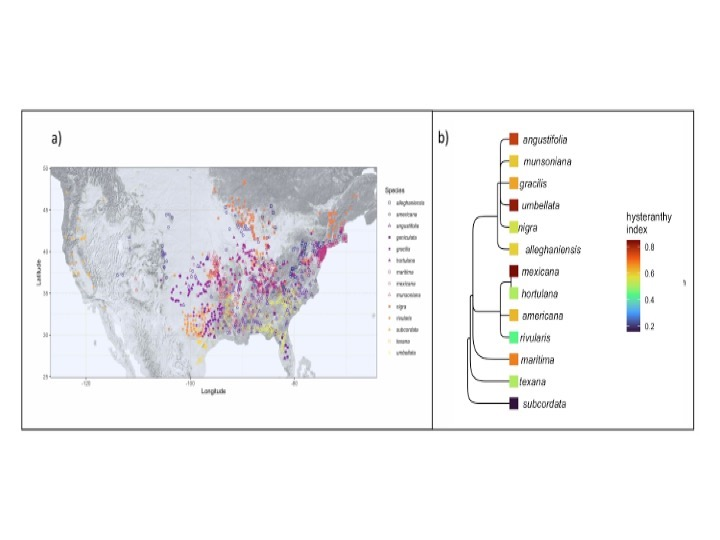
\includegraphics[width=\textwidth]{..//..//Plots/fig1_new.jpg}
    \caption{Geographic distribution and taxonomic relationships among the focal clade Prunocerasus. a) Maps the localities of all the herbaria records used in this study. b) Depicts phylogenetic relationships among the American plums and the duration of their flowering period they are hysteranthous. These categorizations are based on ordinal phylogenetics mixed models. Tree topology is from \citet{Shaw:2004aa}}
    \label{fig:phylo2}
\end{figure}


   % \begin{figure}[h!]
    %\centering
 %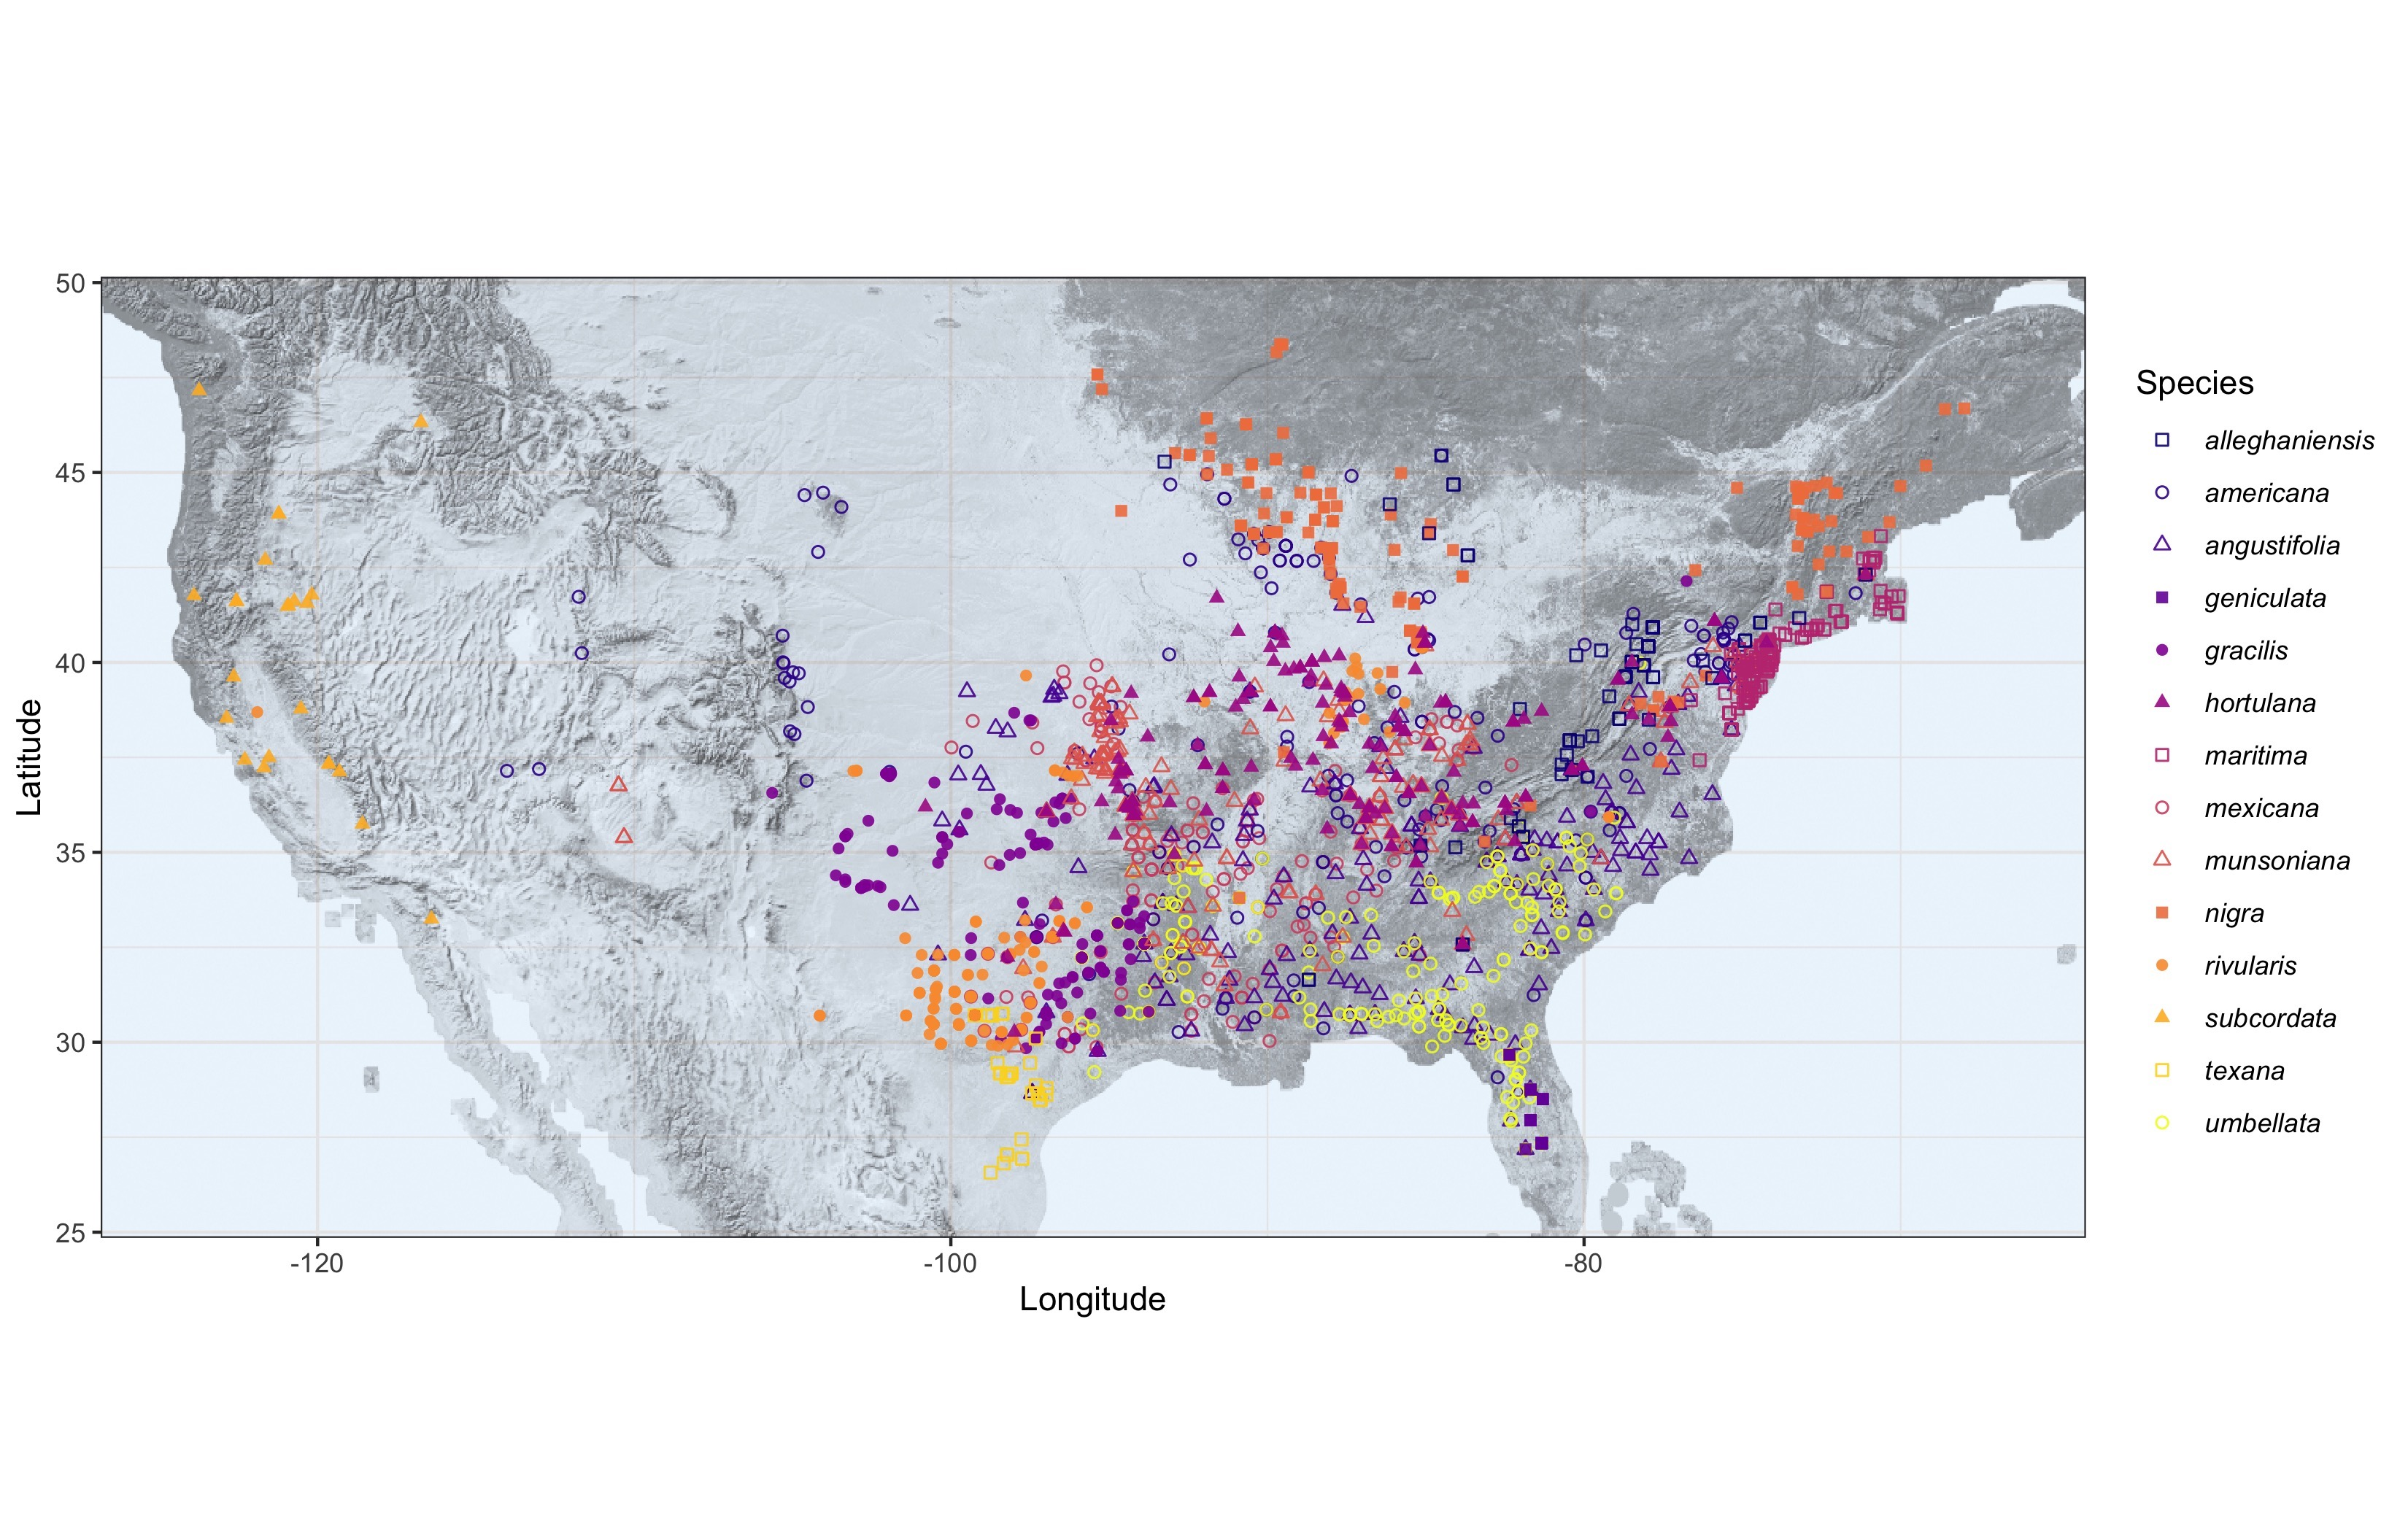
\includegraphics[width=\textwidth]{..//..//Plots/Prunus-Map-raster-plasma.jpeg}
  %  \caption{This is a map of all the herbaria records of our focal clade. Maybe better in the supplement } 
   % \label{fig:mappy}
%\end{figure}

\begin{figure}[h!]
    \centering
 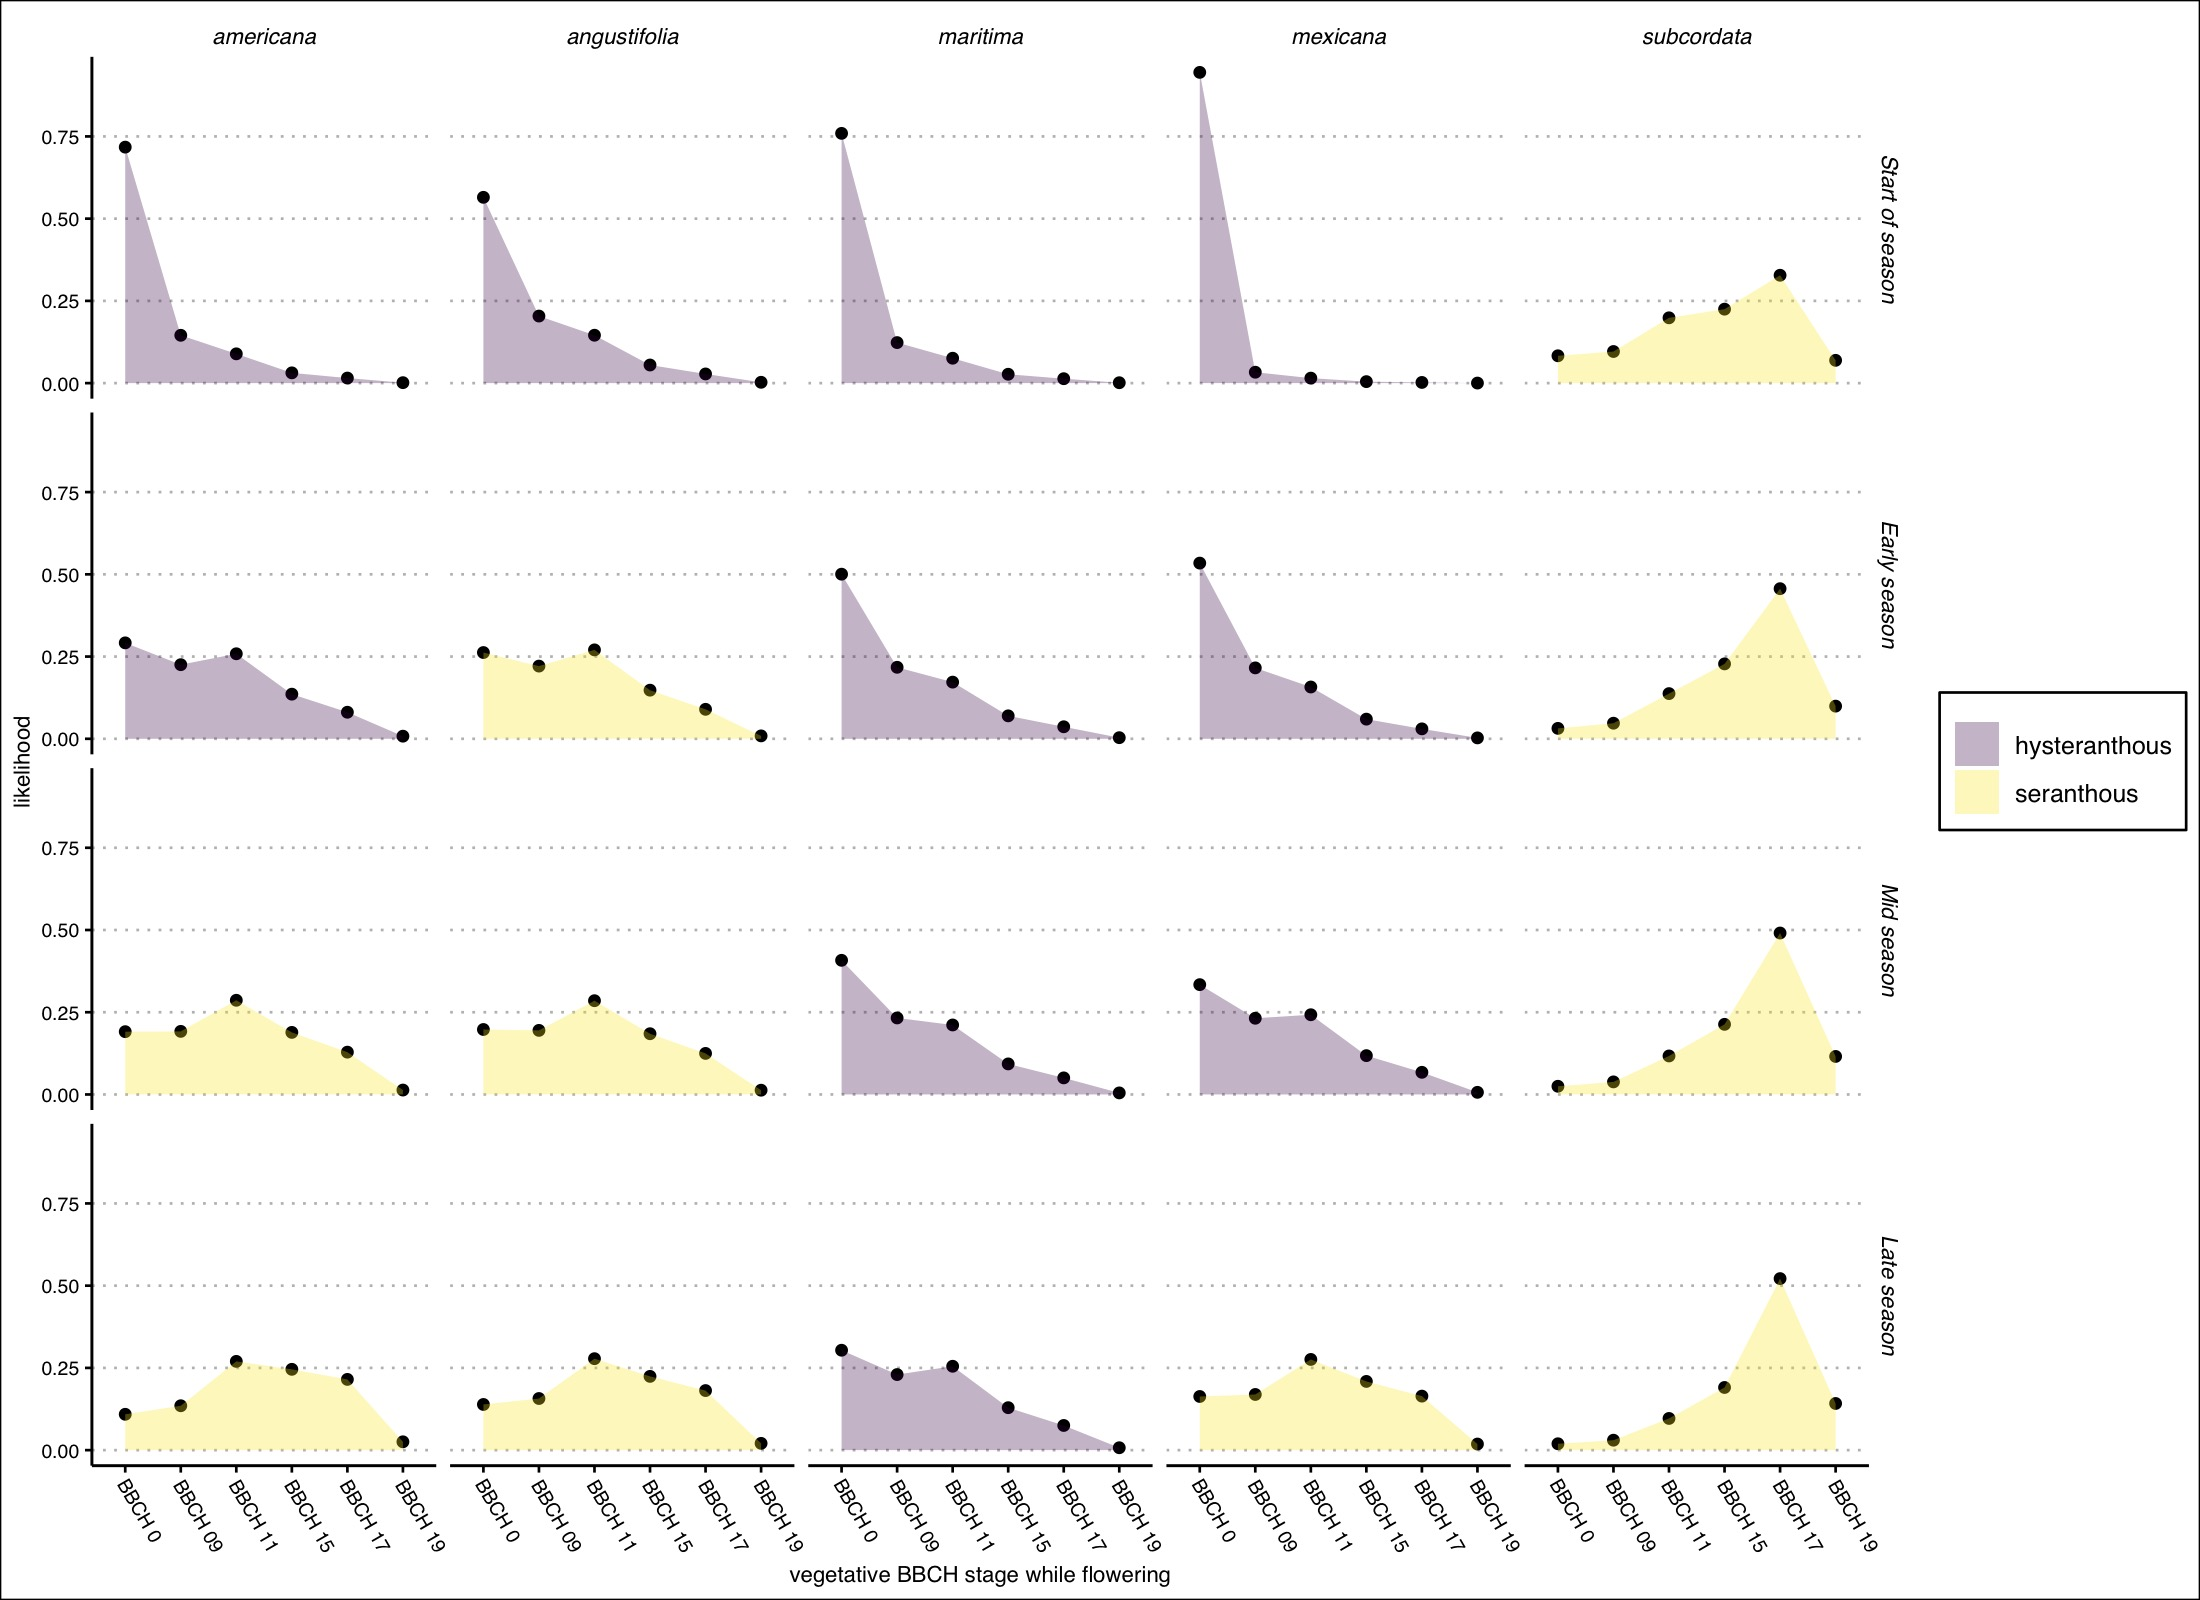
\includegraphics[width=\textwidth]{..//..//Plots/ord_quants_exmpsps.jpeg}
    \caption{Predicted likelihood that a species would be in flower during each vegetative BBCH phase for five example species in the American plums. Points are the mean likelihood and bar the 95\% uncertainty intervals. Species were classified as hysteranthous if greater than 50\% probability flowering occurred in BBCH 0 and BBCH 09 (colors) for each part of the flowering season.
  See Fig. \ref{fig:plums} for all species and alternative hysteranthy classification schemes. }
    \label{fig:ordinals}
\end{figure}



%\begin{figure}[h!]
 %   \centering
 %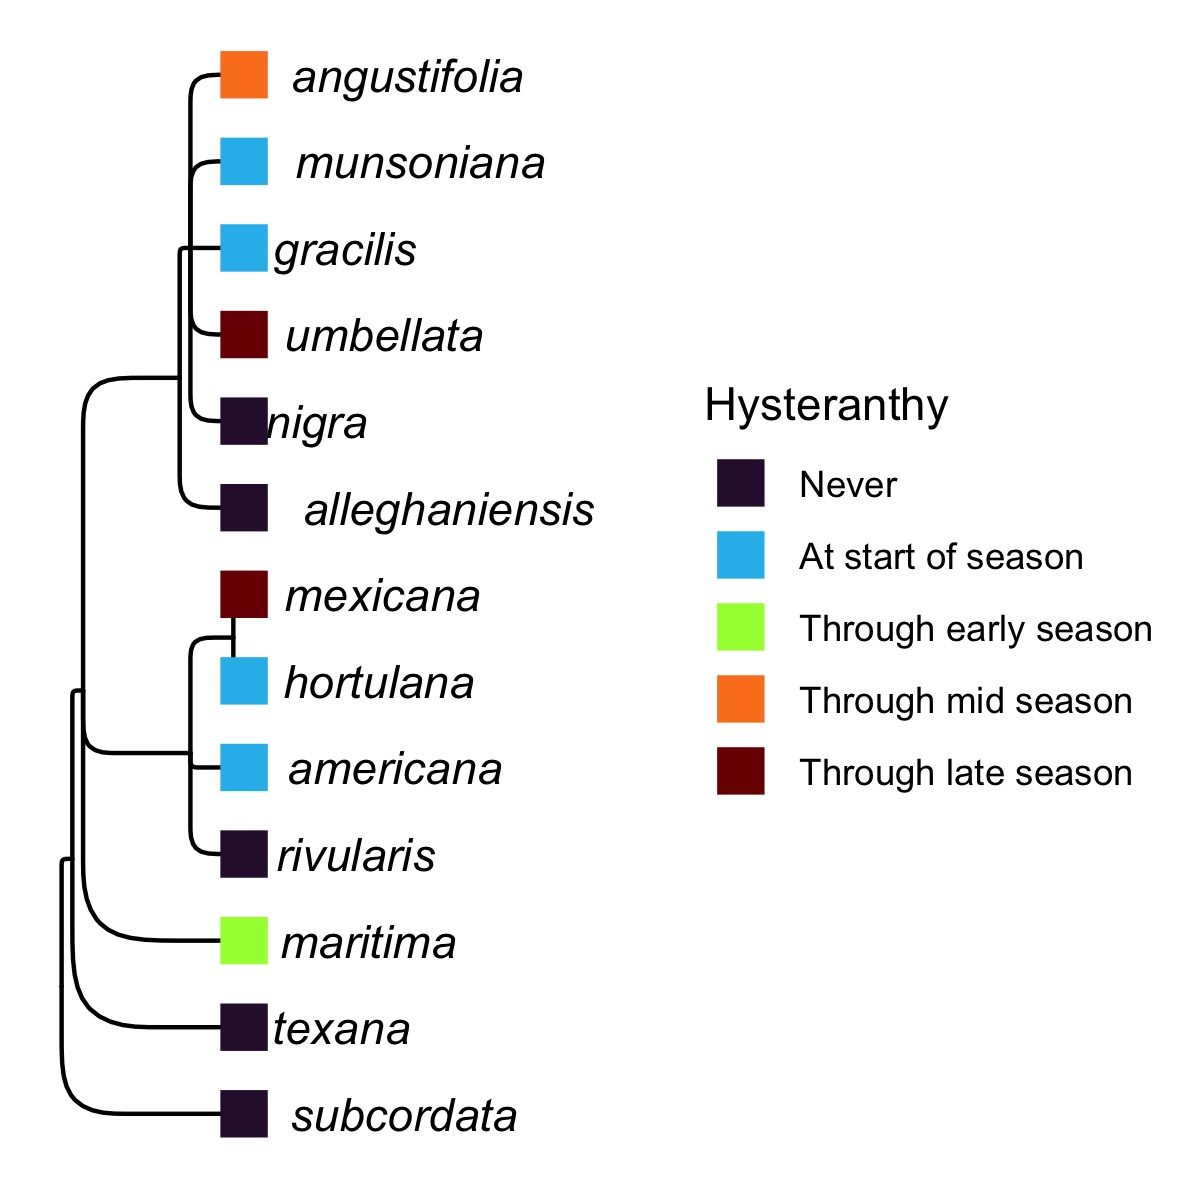
\includegraphics[width=.6\textwidth]{..//..//Plots/phylosig2.jpeg}
  %  \caption{Phylogenetic relationships amoung the American plums and the duration of their flowering perion they are hysterathous. These categorizations are based on ordinal phylogenetics mixed models. Tree topology is from \citet{Shaw:2004aa}}
   % \label{fig:phylo2}
%\end{figure}


\begin{figure}[h!]
    \centering
 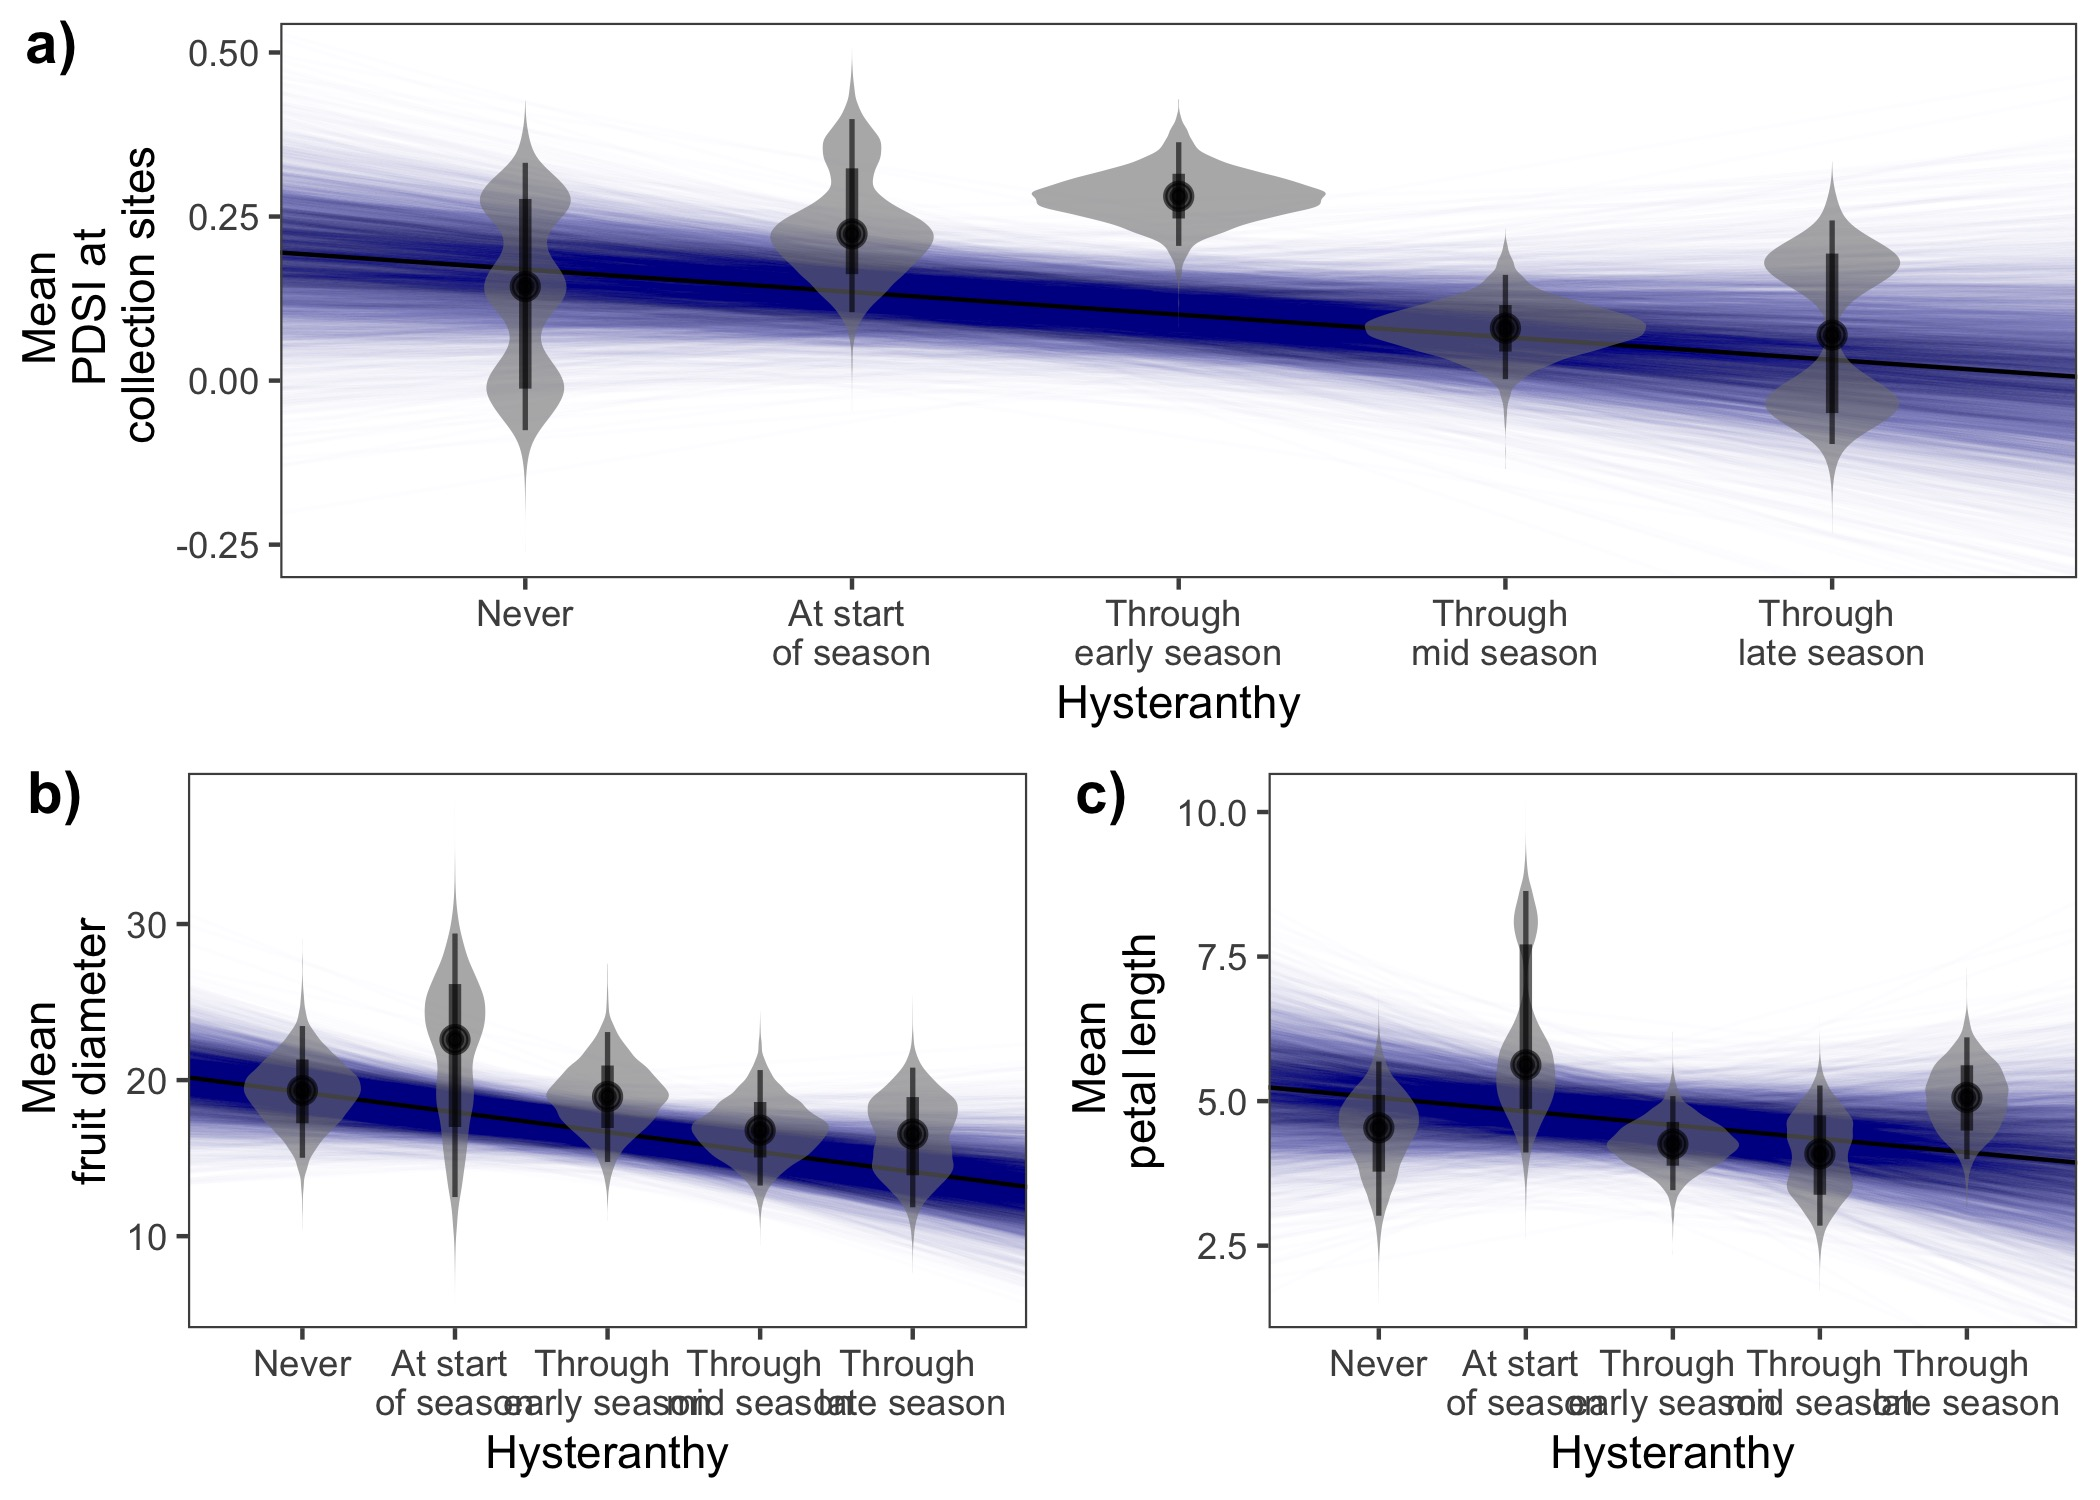
\includegraphics[width=\textwidth]{..//..//Plots/dataplots.jpeg}
    \caption{Relationships between the duration of hysteranthy across the flowering period and environmental and biological traits based on Bayesian phylogenetic mixed models. a) b) and c) dipict the relationships between the duration of hysteranthy and mean PDSI, fruit diameter, and petal length respectively. Solid lines indicate the mean posterior estimate and shaded areas X draws from the posterior distrubtion as a display of uncertainty. }
    \label{fig:prunes}
\end{figure}


\begin{figure}[h!]
    \centering
 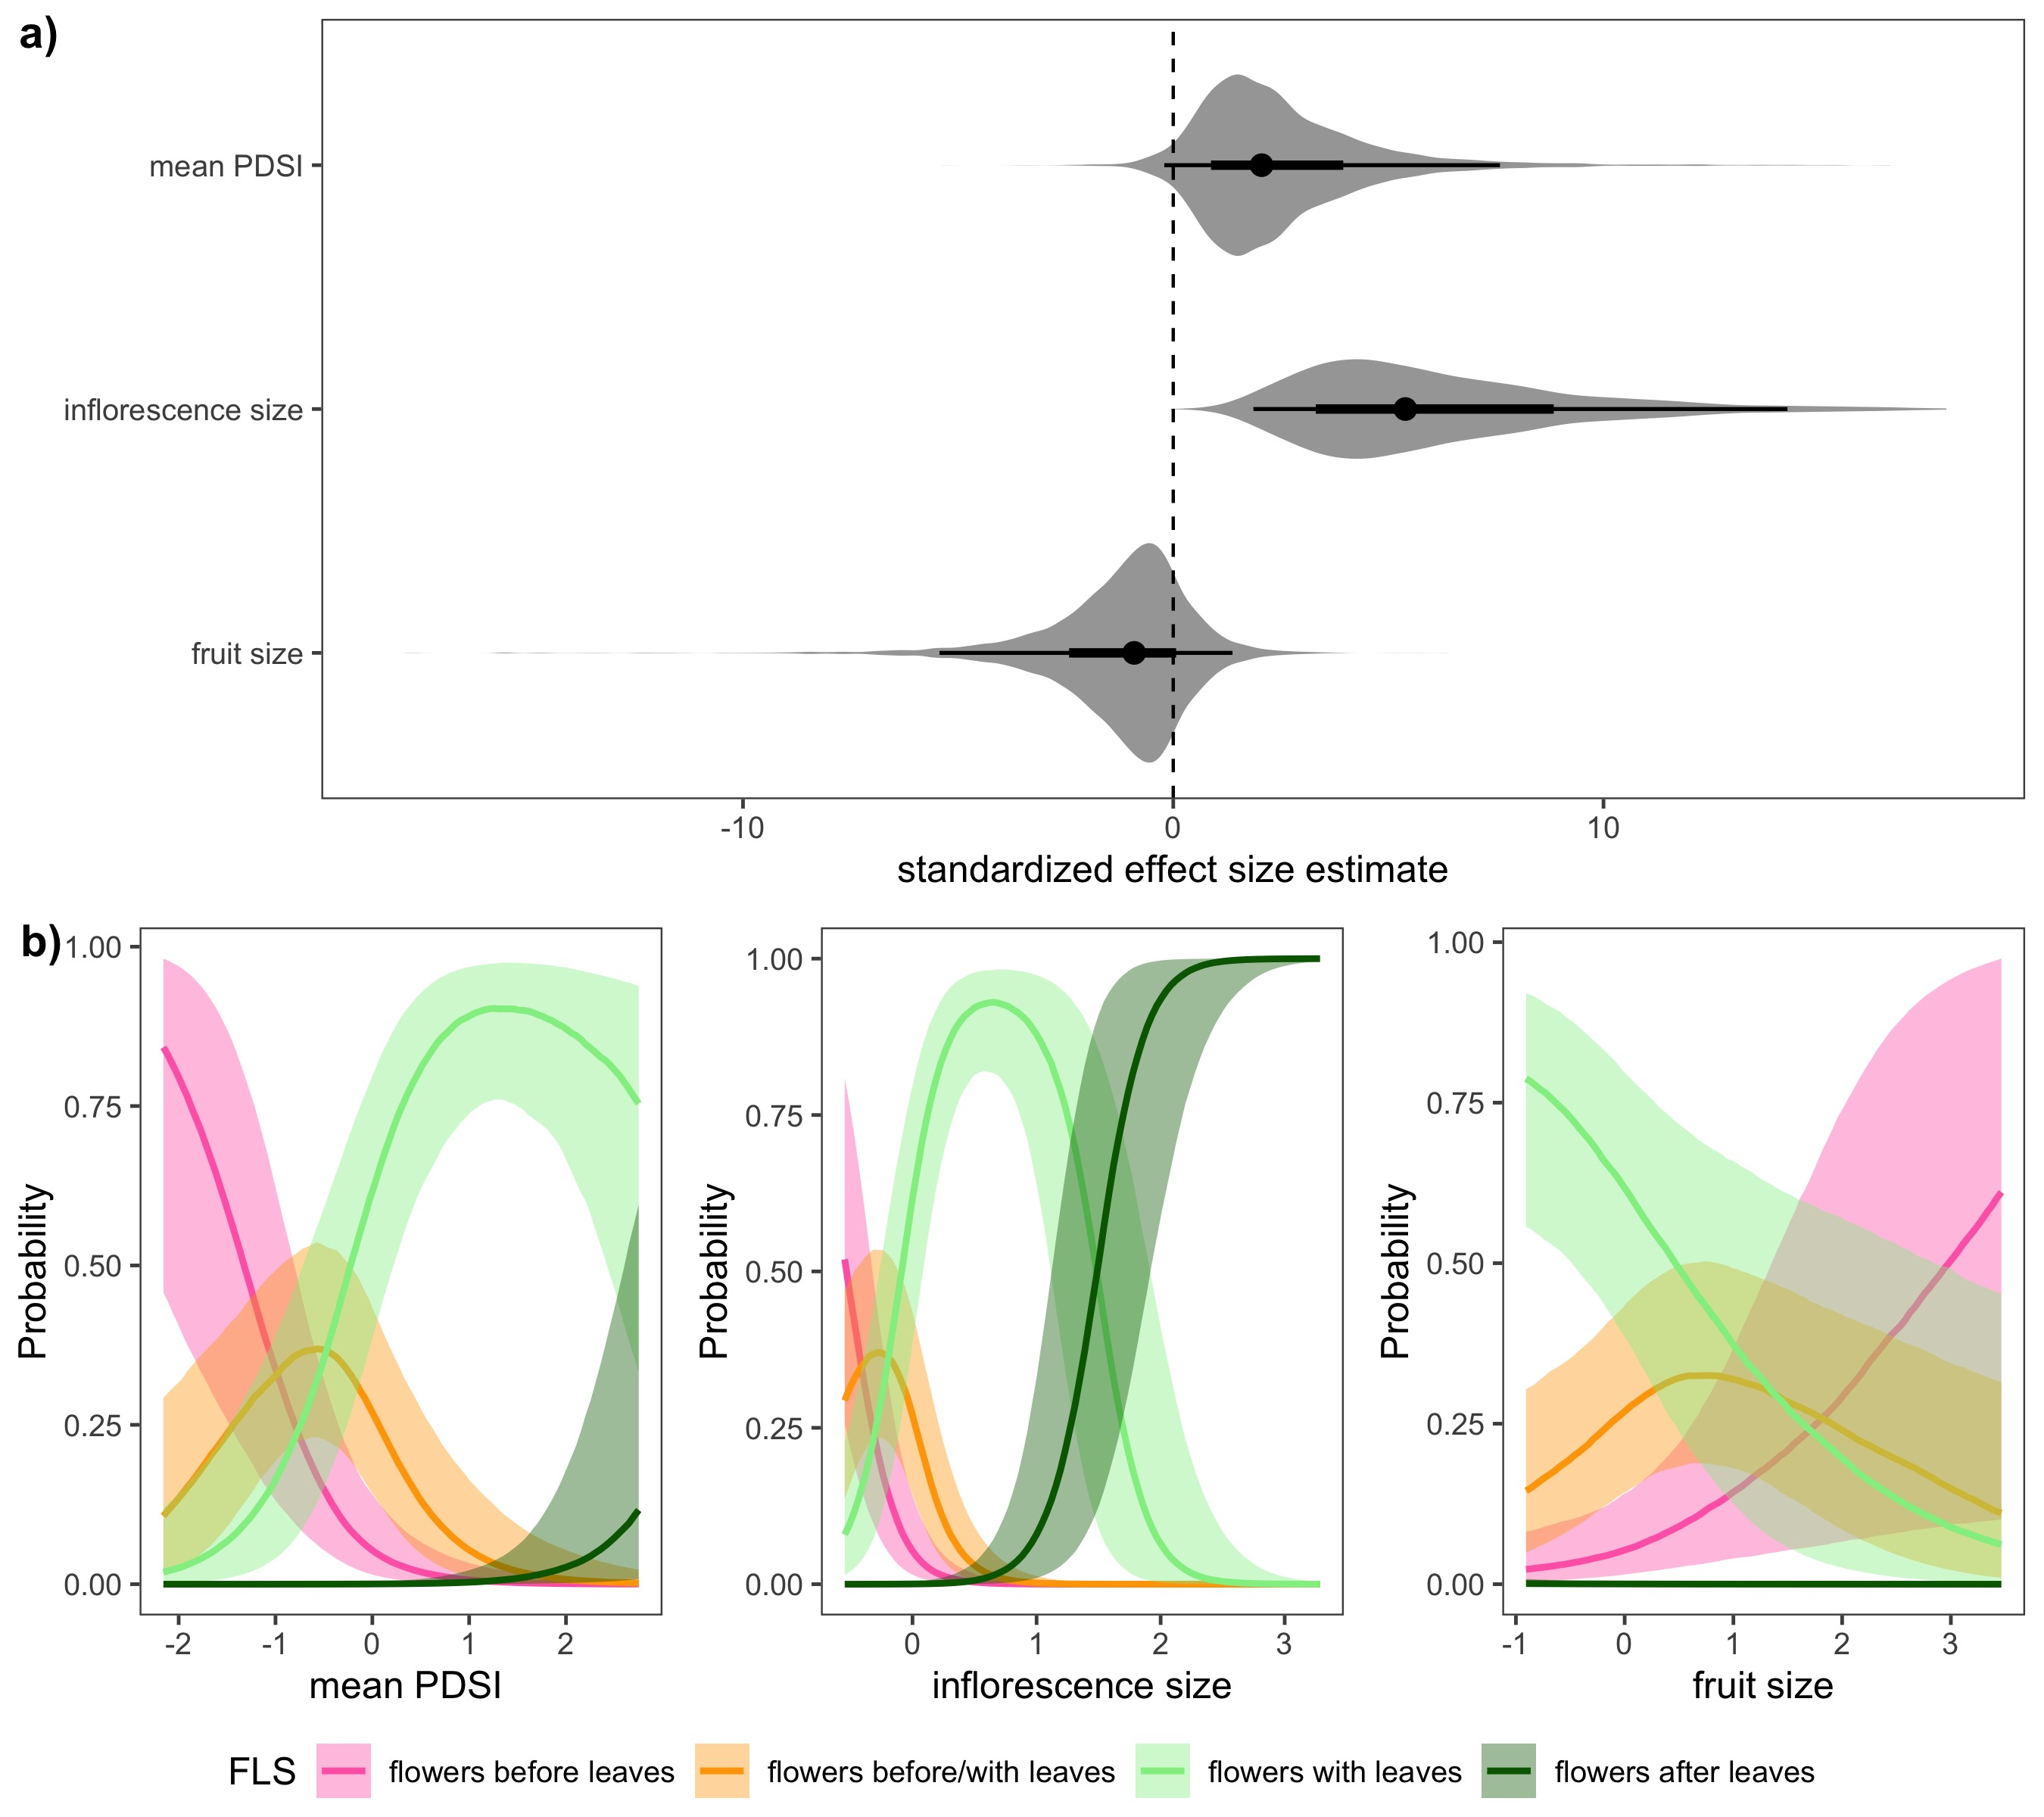
\includegraphics[width=\textwidth]{..//..//Plots/fullprunus_4manu.jpeg} %emwmar9 --mv fruit to supp?
    \caption{Relationships between the likelihood of of hysteranthy and environmental and biological traits in the genus Prunus based on Bayesian phylogenetic mixed models. Panel a) shows the estimated effect size of each predictor with negative values indicating an increased likelihood of hysteranthy. Points indicate the mean posterior estimate for each predictor, and thick and thin bars the 50\% and 97.5\% uncertaintly intervals respectively. We also show the full posterior distribution as an aditional meaure of uncertainty, Panel b), c) and d) show the marginal effect of mean PDSI, inflorescence size and fruit size respectively, on the likelihood that of each FLS category. Solid lines indicate the mean likelihood and shaded areas the 50\% uncertainty intervals.}
    \label{fig:genus}
\end{figure}

%\begin{figure}[h!]
 %   \centering
 %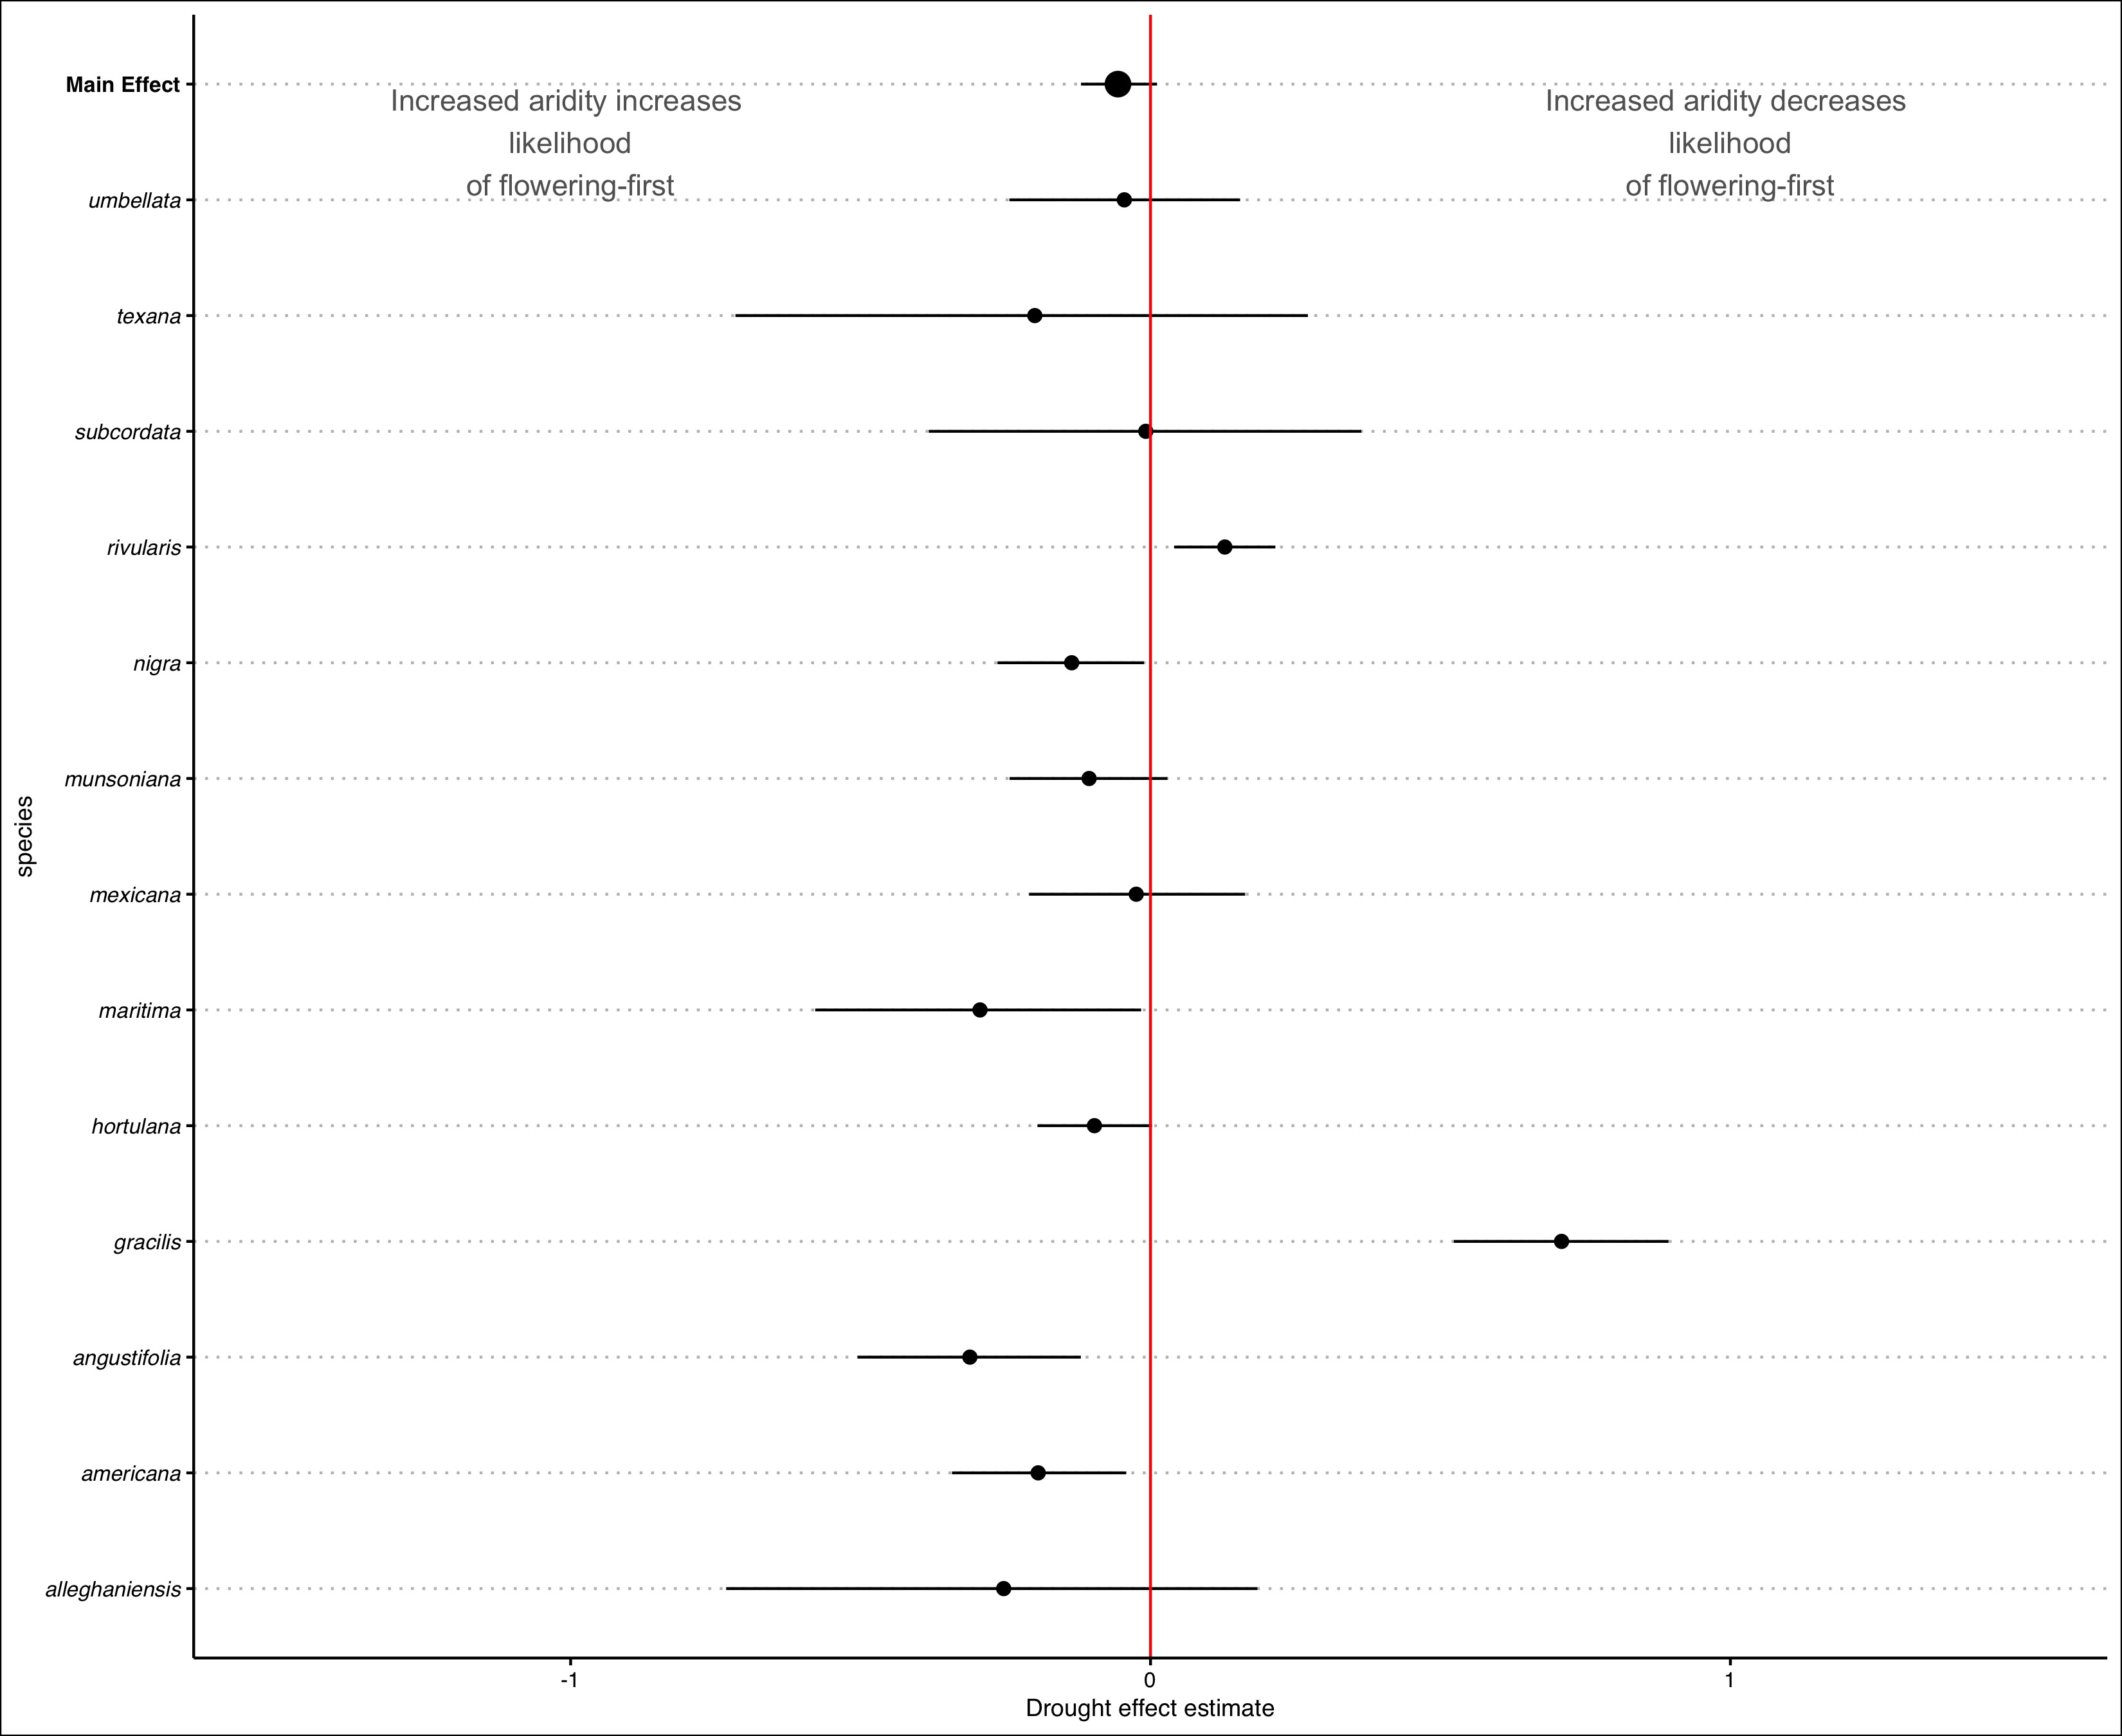
\includegraphics[width=\textwidth]{..//..//Plots/droughtstuff.jpg}
  %  \caption{Hysteranthy more likely in drought years.}
   % \label{fig:plastic}
%\end{figure}

\end{document}
